\documentclass[xcolor=svgnames,9pt,english,aspectratio=169,t]{beamer}
%\documentclass[xcolor=svgnames,9pt,english,handout,aspectratio=169,t]{beamer}
\newcommand{\handout}{0}

% =====================================================================
% POLI 450A (2026) --- shared TEMPLATE layer.
%
% Input from each lecture near the top of its file, BEFORE
% ../course_theme.tex (metropolis must be selected before the course
% palette overrides it):
%
%   \documentclass[xcolor=svgnames,9pt,english,aspectratio=169]{beamer}
%   \newcommand{\handout}{0}
%   % =====================================================================
% POLI 450A (2026) --- shared TEMPLATE layer.
%
% Input from each lecture near the top of its file, BEFORE
% ../course_theme.tex (metropolis must be selected before the course
% palette overrides it):
%
%   \documentclass[xcolor=svgnames,9pt,english,aspectratio=169]{beamer}
%   \newcommand{\handout}{0}
%   % =====================================================================
% POLI 450A (2026) --- shared TEMPLATE layer.
%
% Input from each lecture near the top of its file, BEFORE
% ../course_theme.tex (metropolis must be selected before the course
% palette overrides it):
%
%   \documentclass[xcolor=svgnames,9pt,english,aspectratio=169]{beamer}
%   \newcommand{\handout}{0}
%   \input{../course_preamble.tex}
%   \input{../course_theme.tex}
%   \graphicspath{{./}{./figs/}}
%   \title[Short title]{450A Political Methodology I}
%   \subtitle{Lecture N: ...}
%
% Modeled on the 2026 Northwestern workshop template
% (Teaching/PanelData/_latex/2026/202608_Northwestern/workshop_preamble.tex).
%
% SCOPE: theme, beamer layout, packages, the roadmap hooks, and --- unlike
% the Northwestern decks --- the notation macros. The 450A lectures
% grew from one common ancestor, so their macro blocks agree wherever they
% overlap; merging them is safe. Three points where they had drifted are
% resolved here, and each is flagged inline below.
% =====================================================================

\usetheme{metropolis}
\metroset{sectionpage=none, subsectionpage=none, numbering=none}
\setbeamertemplate{navigation symbols}{}

\setbeamersize{text margin left=5mm, text margin right=5mm}
\setbeamertemplate{itemize/enumerate body begin}{\leftmargini=1.5em\relax}
\setbeamertemplate{itemize/enumerate subbody begin}{\leftmarginii=1.5em\relax}
\setbeamertemplate{itemize/enumerate subsubbody begin}{\leftmarginiii=1.5em\relax}

% ----------------------------------------------------------- top alignment
% Every deck passes the t class option, so beamer applies the frame key
% below to every frame (explicit [plain,c] frames — title page, roadmaps —
% stay centered). Beamer's stock t key puts a rigid .2cm pad above the
% content; frames sized to this template's full-height ceilings then run
% Overfull \vbox by up to that pad. Same key as beamerbaseframe.sty, with
% one change: the pad may shrink to zero when the frame is full.
\makeatletter
\define@key{beamerframe}{t}[true]{% top
  \beamer@frametopskip=.2cm plus .5\paperheight minus .2cm\relax%
  \beamer@framebottomskip=0pt plus 1fill\relax%
  \beamer@frametopskipautobreak=\beamer@frametopskip\relax%
  \beamer@framebottomskipautobreak=\beamer@framebottomskip\relax%
}

% ------------------------------------------------- slide-top check (2026-10-11)
% A slide whose content is too tall for the frame is squeezed: the pad above
% shrinks and its content starts higher than on other slides, so a figure
% "wobbles" when the class steps from one slide to the next (Lecture 4-1,
% slides 1-2, 2026-10-11). The marker below records where each slide's
% content starts (a whatsit: it adds no space and moves nothing).
% `python3 ../check_slides.py lec<N>` then lists every slide that starts
% higher than the deck's normal position. That list must be empty.
% Recorded per slide: page, frame number, content-top y (sp), the room left
% below the title bar, and P for a plain frame (title page, roadmaps).
\providecommand\slidetop[5]{}
\AtBeginDocument{\immediate\write\@auxout{\string\providecommand\string\slidetop[5]{}}}
\def\beamer@markframetop{%
  \pdfsavepos
  \edef\beamer@marktmp{\noexpand\write\noexpand\@auxout{\string\slidetop
    {\noexpand\thepage}{\noexpand\insertframenumber}{\noexpand\the\noexpand\pdflastypos}%
    {\number\beamer@frametextheight}{\ifbeamer@plainframe P\else N\fi}}}%
  \beamer@marktmp}
\RequirePackage{etoolbox}
\patchcmd{\endbeamer@frameslide}
  {\vskip\beamer@frametopskip}
  {\vskip\beamer@frametopskip\beamer@markframetop}
  {}{\PackageWarning{course_preamble}{slide-top marker not installed}}
\makeatother

% ---------------------------------------------------------------- packages
\usepackage{xcolor}
\usepackage{colortbl}
\usepackage{amsmath}
\usepackage{amsfonts}
\usepackage{amssymb}
\usepackage{bm}
\usepackage{graphicx}
\usepackage{multirow}
\usepackage{fancyvrb}
\usepackage{listings}
\usepackage{tikz}
\usetikzlibrary{arrows.meta,positioning,decorations.pathreplacing}

% --------------------------------------------------------- figure fitting
% Default bounding box for every \includegraphics that does not override it.
% With keepaspectratio the image is scaled to fit *inside* width x height, so
% a figure can never run past the side margins or off the bottom of a slide.
% Options given at the call site override these on a per-key basis: e.g.
% [width=.6\linewidth] narrows the box but keeps the height ceiling.
% \figmaxheight is set at \begin{document}: beamer only computes the final
% \textheight once the head/foot templates are known. 0.80 is just under what a
% frame with a title and one line of text can hold (measured: 0.834\textheight);
% a frame that needs more room for text can lower it locally.
\newlength{\figmaxheight}
\AtBeginDocument{\setlength{\figmaxheight}{0.80\textheight}}
\setkeys{Gin}{width=\linewidth,height=\figmaxheight,keepaspectratio}

% -------------------------------------------------------- roadmap frames
% Identical in all lectures. A lecture that does not want the
% subsection roadmap clears it after the \input with \AtBeginSubsection[]{}.
% hideothersubsections is load-bearing, not cosmetic: lecture 4 had 13
% subsections before it was split into 4-1, 4-2 and 4-3 (2026-10-09), and a
% full contents list ran off the top and bottom of the slide. Hiding the other sections' subsections caps the list at 10 lines.
\subject{Talks}
% No back-to-back roadmaps (Yiqing, 2026-10-11): when a subsection starts right
% after its section's roadmap, with no content slide in between, its own
% roadmap would repeat the one just shown (5-1's handout showed "Two Cases"
% twice), so it is skipped. The section roadmap records the frame count; the
% subsection roadmap appears only if a content slide has come since.
\makeatletter
\def\course@secframe{-1}
\AtBeginSection[]
{
  \begin{frame}[plain,c]
    \frametitle{}
    \tableofcontents[currentsection,hideothersubsections]
    \addtocounter{framenumber}{-1}
  \end{frame}
  \xdef\course@secframe{\the\c@framenumber}
}
\AtBeginSubsection[]
{
  \ifnum\c@framenumber=\course@secframe\relax\else
  \begin{frame}[plain,c]
    \frametitle{}
    \tableofcontents[currentsection,currentsubsection,hideothersubsections]
    \addtocounter{framenumber}{-1}
  \end{frame}
  \fi
}
\makeatother

% ------------------------------------------------------ theorem environments
\newtheorem{assumption}{Assumption}
\newtheorem{iass}{Identification Assumption}
\newtheorem{ires}{Identification Result}
\newtheorem{estm}{Estimand}
\newtheorem{esti}{Estimator}
\newtheorem{question}{Question}
\newtheorem{answer}{Answer}
\newtheorem{proposition}{Proposition}

% =====================================================================
% Notation
% =====================================================================
\definecolor{dgreen}{rgb}{0,.6,0.8}

\renewcommand\r{\right}
\renewcommand\l{\left}
\newcommand{\bs}{\boldsymbol}
\newcommand{\mb}{\mathbf}
\newcommand{\real}{\mathbb{R}}
\newcommand{\cN}{\mathcal{N}}
\newcommand{\E}{\mathbb{E}}
\newcommand{\V}{\mathbb{V}}

% MERGE NOTE 1. Lecture 2-4 set \epsilon to \varepsilon; the other twelve
% left it at the upright default. Adopting \varepsilon course-wide so the
% error term looks the same in every lecture.
\renewcommand{\epsilon}{\varepsilon}

% MERGE NOTE 2. Lecture 2-4 wrote its vectors as \bm (bold italic); the other
% twelve use \mathbf (bold upright). \mathbf wins --- it is the convention in
% eleven of the thirteen decks and in the course's matrix lectures. Only
% \iid, \E, \cN and \Var from that block are actually used in 2-4's body.
\renewcommand{\u}{\ensuremath{\mb{u}}}
\renewcommand{\v}{\ensuremath{\mb{v}}}
\newcommand{\U}{\ensuremath{\mb{U}}}
\newcommand{\M}{\ensuremath{\mb{M}}}
\newcommand{\X}{\ensuremath{\mb{X}}}
\newcommand{\x}{\ensuremath{\mb{x}}}
\newcommand{\y}{\ensuremath{\mb{y}}}
\newcommand{\Z}{\ensuremath{\mb{Z}}}
\newcommand{\C}{\ensuremath{\mb{C}}}
\newcommand{\D}{\ensuremath{\mb{D}}}
\newcommand{\I}{\ensuremath{\mb{I}}}
\newcommand{\W}{\ensuremath{\mb{W}}}
\renewcommand{\a}{\ensuremath{\mb{a}}}
\renewcommand{\P}{\ensuremath{\mb{P}}}
\newcommand{\one}{\ensuremath{\mb{1}}}
\newcommand{\zero}{\ensuremath{\mb{0}}}

\renewcommand{\b}{\ensuremath{\bs{\beta}}}
\newcommand{\be}{\ensuremath{\bs{\beta}}}
\newcommand{\e}{\ensuremath{\bs{\epsilon}}}
\newcommand{\eps}{\ensuremath{\bs{\epsilon}}}
\newcommand{\eeta}{\ensuremath{\bs{\eta}}}
\newcommand{\bhat}{\ensuremath{\hat{\bs{\beta}}}}
\newcommand{\ehat}{\ensuremath{\hat{\e}}}
\newcommand{\Sig}{\ensuremath{\bs{\Sigma}}}
\newcommand{\SigInv}{\ensuremath{\bs{\Sigma^{-1}}}}

\newcommand{\XX}{\ensuremath{\X'\X}}
\newcommand{\XXinv}{\ensuremath{\left(\XX\right)^{-1}}}
\newcommand{\hatmat}{\ensuremath{\X \XXinv \X'}}
\newcommand{\hatsig}{\ensuremath{\hat{\sigma}^2}}
\newcommand{\sig}{\ensuremath{\sigma^2}}

\newcommand{\cA}{\mathcal{A}}
\newcommand{\cJ}{\mathcal{J}}
\newcommand{\cL}{\mathcal{L}}
\newcommand{\cLL}{\mathcal{LL}}
\newcommand{\cll}{\ell}
\newcommand{\cQ}{\mathcal{Q}}
\newcommand{\cP}{\mathcal{P}}

% MERGE NOTE 3. \var / \Var and \cov / \Cov were spelled with \text in some
% lectures and \mbox in others. Same output; \text kept.
\newcommand{\var}{\text{Var}}
\newcommand{\Var}{\text{Var}}
\newcommand{\cov}{\text{Cov}}
\newcommand{\Cov}{\text{Cov}}
\newcommand{\cor}{\text{Cor}}
\newcommand{\tr}{\text{tr}}
\newcommand{\avepop}{\frac{1}{n}\sum_{i=1}^n}

\DeclareMathOperator*\plim{plim}
\DeclareMathOperator\rank{rank}
\DeclareMathOperator*\argmax{argmax}
\DeclareMathOperator*\argmin{argmin}
\DeclareMathOperator{\sgn}{sgn}
\newcommand{\diag}{\mathop{\mathrm{diag}}}

\newcommand\ud{\mathrm{d}}
\newcommand\dist{\buildrel\rm d\over\sim}
\newcommand\ind{\stackrel{\rm indep.}{\sim}}
\newcommand\iid{\stackrel{\rm i.i.d.}{\sim}}
\newcommand\logit{{\rm logit}}

\newcommand\indep{\protect\mathpalette{\protect\independenT}{\perp}}
\def\independenT#1#2{\mathrel{\rlap{$#1#2$}\mkern2mu{#1#2}}}

% ------------------------------------------------------------- text helpers
\newcommand{\bi}{\begin{itemize}}
\newcommand{\ei}{\end{itemize}}
\newcommand{\noi}{\noindent}
\newcommand{\red}{\textcolor{Cardinal}}
\newcommand{\blue}{\textcolor{CourseBlue}}
\newcommand{\gray}{\textcolor{gray}}
\newcommand\spacingset[1]{\renewcommand{\baselinestretch}{#1}\small\normalsize}

\hyphenation{tyamamot}


% ------------------------------------------------ figure-position check (2026-10-11)
% Records where every \includegraphics lands and its size (a whatsit; it moves
% nothing). check_slides.py flags two consecutive slides that show a figure of
% the same size in different places: the class sees it jump (Lecture 3, slides
% 18 to 19: one frame had \vspace{.3cm} above the figure, the next did not),
% and two consecutive slides that show the same file at different sizes or
% places (Lecture 6-3, slides 10 to 11, the ballot image). The file name is the
% seventh field.
\makeatletter
\providecommand\figpos[7]{}
\AtBeginDocument{\immediate\write\@auxout{\string\providecommand\string\figpos[7]{}}}
\newbox\course@figbox
\let\course@origGinclude\Ginclude@graphics
\def\Ginclude@graphics#1{%
  \setbox\course@figbox\hbox{\course@origGinclude{#1}}%
  \pdfsavepos
  \edef\course@figtmp{\noexpand\write\noexpand\@auxout{\string\figpos
    {\noexpand\thepage}{\noexpand\insertframenumber}%
    {\noexpand\the\noexpand\pdflastxpos}{\noexpand\the\noexpand\pdflastypos}%
    {\number\wd\course@figbox}{\number\ht\course@figbox}{\detokenize{#1}}}}%
  \course@figtmp
  \box\course@figbox}
\makeatother

%   % =====================================================================
% POLI 450A (2026) --- shared visual system.
% Input from each lecture AFTER ../course_preamble.tex.
%
% Same shape as the 2026 Northwestern workshop theme
% (Teaching/PanelData/_latex/2026/202608_Northwestern/workshop_theme.tex),
% with the workshop's purple swapped for the course's cardinal. Kept
% deliberately light so the lecture sources stay easy to edit.
%
% To retune the course to Stanford's official cardinal, change the one
% Cardinal line below to HTML 8C1515.
% =====================================================================
\definecolor{Cardinal}{HTML}{A8003B}     % primary: titles, structure, alerts
\definecolor{CourseInk}{HTML}{252A34}    % body text
\definecolor{CourseBlue}{HTML}{2F6B9A}   % secondary accent
\definecolor{CourseMist}{HTML}{F8F1F4}   % block backgrounds

\setbeamercolor{normal text}{fg=CourseInk,bg=white}
\setbeamercolor{structure}{fg=Cardinal}
\setbeamercolor{alerted text}{fg=Cardinal}
\setbeamercolor{frametitle}{fg=white,bg=Cardinal}
\setbeamercolor{title}{fg=Cardinal}
\setbeamercolor{subtitle}{fg=CourseInk}
\setbeamercolor{block title}{fg=white,bg=Cardinal}
\setbeamercolor{block body}{fg=CourseInk,bg=CourseMist}
\setbeamercolor{section in toc}{fg=Cardinal}
\setbeamercolor{subsection in toc}{fg=CourseInk}
\setbeamercolor{itemize item}{fg=Cardinal}
\setbeamercolor{itemize subitem}{fg=Cardinal}
\setbeamercolor{enumerate item}{fg=Cardinal}

\setbeamerfont{title}{series=\bfseries,size=\Large}
\setbeamerfont{frametitle}{series=\bfseries,size=\large}
\setbeamerfont{block title}{series=\bfseries}
\setbeamertemplate{navigation symbols}{}
\setbeamertemplate{items}[circle]
\setbeamertemplate{blocks}[rounded][shadow=false]
\setbeamertemplate{frametitle continuation}{}
\setbeamertemplate{footline}{%
  \leavevmode\hbox{%
  \begin{beamercolorbox}[wd=.88\paperwidth,ht=2.6ex,dp=1.2ex,leftskip=1.2em]{author in head/foot}%
  \usebeamerfont{author in head/foot}\insertshorttitle
  \end{beamercolorbox}%
  \begin{beamercolorbox}[wd=.12\paperwidth,ht=2.6ex,dp=1.2ex,center]{date in head/foot}%
  \insertframenumber
  \end{beamercolorbox}}}

\newcommand{\slidesource}[1]{\vfill{\scriptsize\color{gray}Source: #1}}
\newcommand{\keyquestion}[1]{\begin{block}{Question}#1\end{block}}

%   \graphicspath{{./}{./figs/}}
%   \title[Short title]{450A Political Methodology I}
%   \subtitle{Lecture N: ...}
%
% Modeled on the 2026 Northwestern workshop template
% (Teaching/PanelData/_latex/2026/202608_Northwestern/workshop_preamble.tex).
%
% SCOPE: theme, beamer layout, packages, the roadmap hooks, and --- unlike
% the Northwestern decks --- the notation macros. The 450A lectures
% grew from one common ancestor, so their macro blocks agree wherever they
% overlap; merging them is safe. Three points where they had drifted are
% resolved here, and each is flagged inline below.
% =====================================================================

\usetheme{metropolis}
\metroset{sectionpage=none, subsectionpage=none, numbering=none}
\setbeamertemplate{navigation symbols}{}

\setbeamersize{text margin left=5mm, text margin right=5mm}
\setbeamertemplate{itemize/enumerate body begin}{\leftmargini=1.5em\relax}
\setbeamertemplate{itemize/enumerate subbody begin}{\leftmarginii=1.5em\relax}
\setbeamertemplate{itemize/enumerate subsubbody begin}{\leftmarginiii=1.5em\relax}

% ----------------------------------------------------------- top alignment
% Every deck passes the t class option, so beamer applies the frame key
% below to every frame (explicit [plain,c] frames — title page, roadmaps —
% stay centered). Beamer's stock t key puts a rigid .2cm pad above the
% content; frames sized to this template's full-height ceilings then run
% Overfull \vbox by up to that pad. Same key as beamerbaseframe.sty, with
% one change: the pad may shrink to zero when the frame is full.
\makeatletter
\define@key{beamerframe}{t}[true]{% top
  \beamer@frametopskip=.2cm plus .5\paperheight minus .2cm\relax%
  \beamer@framebottomskip=0pt plus 1fill\relax%
  \beamer@frametopskipautobreak=\beamer@frametopskip\relax%
  \beamer@framebottomskipautobreak=\beamer@framebottomskip\relax%
}

% ------------------------------------------------- slide-top check (2026-10-11)
% A slide whose content is too tall for the frame is squeezed: the pad above
% shrinks and its content starts higher than on other slides, so a figure
% "wobbles" when the class steps from one slide to the next (Lecture 4-1,
% slides 1-2, 2026-10-11). The marker below records where each slide's
% content starts (a whatsit: it adds no space and moves nothing).
% `python3 ../check_slides.py lec<N>` then lists every slide that starts
% higher than the deck's normal position. That list must be empty.
% Recorded per slide: page, frame number, content-top y (sp), the room left
% below the title bar, and P for a plain frame (title page, roadmaps).
\providecommand\slidetop[5]{}
\AtBeginDocument{\immediate\write\@auxout{\string\providecommand\string\slidetop[5]{}}}
\def\beamer@markframetop{%
  \pdfsavepos
  \edef\beamer@marktmp{\noexpand\write\noexpand\@auxout{\string\slidetop
    {\noexpand\thepage}{\noexpand\insertframenumber}{\noexpand\the\noexpand\pdflastypos}%
    {\number\beamer@frametextheight}{\ifbeamer@plainframe P\else N\fi}}}%
  \beamer@marktmp}
\RequirePackage{etoolbox}
\patchcmd{\endbeamer@frameslide}
  {\vskip\beamer@frametopskip}
  {\vskip\beamer@frametopskip\beamer@markframetop}
  {}{\PackageWarning{course_preamble}{slide-top marker not installed}}
\makeatother

% ---------------------------------------------------------------- packages
\usepackage{xcolor}
\usepackage{colortbl}
\usepackage{amsmath}
\usepackage{amsfonts}
\usepackage{amssymb}
\usepackage{bm}
\usepackage{graphicx}
\usepackage{multirow}
\usepackage{fancyvrb}
\usepackage{listings}
\usepackage{tikz}
\usetikzlibrary{arrows.meta,positioning,decorations.pathreplacing}

% --------------------------------------------------------- figure fitting
% Default bounding box for every \includegraphics that does not override it.
% With keepaspectratio the image is scaled to fit *inside* width x height, so
% a figure can never run past the side margins or off the bottom of a slide.
% Options given at the call site override these on a per-key basis: e.g.
% [width=.6\linewidth] narrows the box but keeps the height ceiling.
% \figmaxheight is set at \begin{document}: beamer only computes the final
% \textheight once the head/foot templates are known. 0.80 is just under what a
% frame with a title and one line of text can hold (measured: 0.834\textheight);
% a frame that needs more room for text can lower it locally.
\newlength{\figmaxheight}
\AtBeginDocument{\setlength{\figmaxheight}{0.80\textheight}}
\setkeys{Gin}{width=\linewidth,height=\figmaxheight,keepaspectratio}

% -------------------------------------------------------- roadmap frames
% Identical in all lectures. A lecture that does not want the
% subsection roadmap clears it after the \input with \AtBeginSubsection[]{}.
% hideothersubsections is load-bearing, not cosmetic: lecture 4 had 13
% subsections before it was split into 4-1, 4-2 and 4-3 (2026-10-09), and a
% full contents list ran off the top and bottom of the slide. Hiding the other sections' subsections caps the list at 10 lines.
\subject{Talks}
% No back-to-back roadmaps (Yiqing, 2026-10-11): when a subsection starts right
% after its section's roadmap, with no content slide in between, its own
% roadmap would repeat the one just shown (5-1's handout showed "Two Cases"
% twice), so it is skipped. The section roadmap records the frame count; the
% subsection roadmap appears only if a content slide has come since.
\makeatletter
\def\course@secframe{-1}
\AtBeginSection[]
{
  \begin{frame}[plain,c]
    \frametitle{}
    \tableofcontents[currentsection,hideothersubsections]
    \addtocounter{framenumber}{-1}
  \end{frame}
  \xdef\course@secframe{\the\c@framenumber}
}
\AtBeginSubsection[]
{
  \ifnum\c@framenumber=\course@secframe\relax\else
  \begin{frame}[plain,c]
    \frametitle{}
    \tableofcontents[currentsection,currentsubsection,hideothersubsections]
    \addtocounter{framenumber}{-1}
  \end{frame}
  \fi
}
\makeatother

% ------------------------------------------------------ theorem environments
\newtheorem{assumption}{Assumption}
\newtheorem{iass}{Identification Assumption}
\newtheorem{ires}{Identification Result}
\newtheorem{estm}{Estimand}
\newtheorem{esti}{Estimator}
\newtheorem{question}{Question}
\newtheorem{answer}{Answer}
\newtheorem{proposition}{Proposition}

% =====================================================================
% Notation
% =====================================================================
\definecolor{dgreen}{rgb}{0,.6,0.8}

\renewcommand\r{\right}
\renewcommand\l{\left}
\newcommand{\bs}{\boldsymbol}
\newcommand{\mb}{\mathbf}
\newcommand{\real}{\mathbb{R}}
\newcommand{\cN}{\mathcal{N}}
\newcommand{\E}{\mathbb{E}}
\newcommand{\V}{\mathbb{V}}

% MERGE NOTE 1. Lecture 2-4 set \epsilon to \varepsilon; the other twelve
% left it at the upright default. Adopting \varepsilon course-wide so the
% error term looks the same in every lecture.
\renewcommand{\epsilon}{\varepsilon}

% MERGE NOTE 2. Lecture 2-4 wrote its vectors as \bm (bold italic); the other
% twelve use \mathbf (bold upright). \mathbf wins --- it is the convention in
% eleven of the thirteen decks and in the course's matrix lectures. Only
% \iid, \E, \cN and \Var from that block are actually used in 2-4's body.
\renewcommand{\u}{\ensuremath{\mb{u}}}
\renewcommand{\v}{\ensuremath{\mb{v}}}
\newcommand{\U}{\ensuremath{\mb{U}}}
\newcommand{\M}{\ensuremath{\mb{M}}}
\newcommand{\X}{\ensuremath{\mb{X}}}
\newcommand{\x}{\ensuremath{\mb{x}}}
\newcommand{\y}{\ensuremath{\mb{y}}}
\newcommand{\Z}{\ensuremath{\mb{Z}}}
\newcommand{\C}{\ensuremath{\mb{C}}}
\newcommand{\D}{\ensuremath{\mb{D}}}
\newcommand{\I}{\ensuremath{\mb{I}}}
\newcommand{\W}{\ensuremath{\mb{W}}}
\renewcommand{\a}{\ensuremath{\mb{a}}}
\renewcommand{\P}{\ensuremath{\mb{P}}}
\newcommand{\one}{\ensuremath{\mb{1}}}
\newcommand{\zero}{\ensuremath{\mb{0}}}

\renewcommand{\b}{\ensuremath{\bs{\beta}}}
\newcommand{\be}{\ensuremath{\bs{\beta}}}
\newcommand{\e}{\ensuremath{\bs{\epsilon}}}
\newcommand{\eps}{\ensuremath{\bs{\epsilon}}}
\newcommand{\eeta}{\ensuremath{\bs{\eta}}}
\newcommand{\bhat}{\ensuremath{\hat{\bs{\beta}}}}
\newcommand{\ehat}{\ensuremath{\hat{\e}}}
\newcommand{\Sig}{\ensuremath{\bs{\Sigma}}}
\newcommand{\SigInv}{\ensuremath{\bs{\Sigma^{-1}}}}

\newcommand{\XX}{\ensuremath{\X'\X}}
\newcommand{\XXinv}{\ensuremath{\left(\XX\right)^{-1}}}
\newcommand{\hatmat}{\ensuremath{\X \XXinv \X'}}
\newcommand{\hatsig}{\ensuremath{\hat{\sigma}^2}}
\newcommand{\sig}{\ensuremath{\sigma^2}}

\newcommand{\cA}{\mathcal{A}}
\newcommand{\cJ}{\mathcal{J}}
\newcommand{\cL}{\mathcal{L}}
\newcommand{\cLL}{\mathcal{LL}}
\newcommand{\cll}{\ell}
\newcommand{\cQ}{\mathcal{Q}}
\newcommand{\cP}{\mathcal{P}}

% MERGE NOTE 3. \var / \Var and \cov / \Cov were spelled with \text in some
% lectures and \mbox in others. Same output; \text kept.
\newcommand{\var}{\text{Var}}
\newcommand{\Var}{\text{Var}}
\newcommand{\cov}{\text{Cov}}
\newcommand{\Cov}{\text{Cov}}
\newcommand{\cor}{\text{Cor}}
\newcommand{\tr}{\text{tr}}
\newcommand{\avepop}{\frac{1}{n}\sum_{i=1}^n}

\DeclareMathOperator*\plim{plim}
\DeclareMathOperator\rank{rank}
\DeclareMathOperator*\argmax{argmax}
\DeclareMathOperator*\argmin{argmin}
\DeclareMathOperator{\sgn}{sgn}
\newcommand{\diag}{\mathop{\mathrm{diag}}}

\newcommand\ud{\mathrm{d}}
\newcommand\dist{\buildrel\rm d\over\sim}
\newcommand\ind{\stackrel{\rm indep.}{\sim}}
\newcommand\iid{\stackrel{\rm i.i.d.}{\sim}}
\newcommand\logit{{\rm logit}}

\newcommand\indep{\protect\mathpalette{\protect\independenT}{\perp}}
\def\independenT#1#2{\mathrel{\rlap{$#1#2$}\mkern2mu{#1#2}}}

% ------------------------------------------------------------- text helpers
\newcommand{\bi}{\begin{itemize}}
\newcommand{\ei}{\end{itemize}}
\newcommand{\noi}{\noindent}
\newcommand{\red}{\textcolor{Cardinal}}
\newcommand{\blue}{\textcolor{CourseBlue}}
\newcommand{\gray}{\textcolor{gray}}
\newcommand\spacingset[1]{\renewcommand{\baselinestretch}{#1}\small\normalsize}

\hyphenation{tyamamot}


% ------------------------------------------------ figure-position check (2026-10-11)
% Records where every \includegraphics lands and its size (a whatsit; it moves
% nothing). check_slides.py flags two consecutive slides that show a figure of
% the same size in different places: the class sees it jump (Lecture 3, slides
% 18 to 19: one frame had \vspace{.3cm} above the figure, the next did not),
% and two consecutive slides that show the same file at different sizes or
% places (Lecture 6-3, slides 10 to 11, the ballot image). The file name is the
% seventh field.
\makeatletter
\providecommand\figpos[7]{}
\AtBeginDocument{\immediate\write\@auxout{\string\providecommand\string\figpos[7]{}}}
\newbox\course@figbox
\let\course@origGinclude\Ginclude@graphics
\def\Ginclude@graphics#1{%
  \setbox\course@figbox\hbox{\course@origGinclude{#1}}%
  \pdfsavepos
  \edef\course@figtmp{\noexpand\write\noexpand\@auxout{\string\figpos
    {\noexpand\thepage}{\noexpand\insertframenumber}%
    {\noexpand\the\noexpand\pdflastxpos}{\noexpand\the\noexpand\pdflastypos}%
    {\number\wd\course@figbox}{\number\ht\course@figbox}{\detokenize{#1}}}}%
  \course@figtmp
  \box\course@figbox}
\makeatother

%   % =====================================================================
% POLI 450A (2026) --- shared visual system.
% Input from each lecture AFTER ../course_preamble.tex.
%
% Same shape as the 2026 Northwestern workshop theme
% (Teaching/PanelData/_latex/2026/202608_Northwestern/workshop_theme.tex),
% with the workshop's purple swapped for the course's cardinal. Kept
% deliberately light so the lecture sources stay easy to edit.
%
% To retune the course to Stanford's official cardinal, change the one
% Cardinal line below to HTML 8C1515.
% =====================================================================
\definecolor{Cardinal}{HTML}{A8003B}     % primary: titles, structure, alerts
\definecolor{CourseInk}{HTML}{252A34}    % body text
\definecolor{CourseBlue}{HTML}{2F6B9A}   % secondary accent
\definecolor{CourseMist}{HTML}{F8F1F4}   % block backgrounds

\setbeamercolor{normal text}{fg=CourseInk,bg=white}
\setbeamercolor{structure}{fg=Cardinal}
\setbeamercolor{alerted text}{fg=Cardinal}
\setbeamercolor{frametitle}{fg=white,bg=Cardinal}
\setbeamercolor{title}{fg=Cardinal}
\setbeamercolor{subtitle}{fg=CourseInk}
\setbeamercolor{block title}{fg=white,bg=Cardinal}
\setbeamercolor{block body}{fg=CourseInk,bg=CourseMist}
\setbeamercolor{section in toc}{fg=Cardinal}
\setbeamercolor{subsection in toc}{fg=CourseInk}
\setbeamercolor{itemize item}{fg=Cardinal}
\setbeamercolor{itemize subitem}{fg=Cardinal}
\setbeamercolor{enumerate item}{fg=Cardinal}

\setbeamerfont{title}{series=\bfseries,size=\Large}
\setbeamerfont{frametitle}{series=\bfseries,size=\large}
\setbeamerfont{block title}{series=\bfseries}
\setbeamertemplate{navigation symbols}{}
\setbeamertemplate{items}[circle]
\setbeamertemplate{blocks}[rounded][shadow=false]
\setbeamertemplate{frametitle continuation}{}
\setbeamertemplate{footline}{%
  \leavevmode\hbox{%
  \begin{beamercolorbox}[wd=.88\paperwidth,ht=2.6ex,dp=1.2ex,leftskip=1.2em]{author in head/foot}%
  \usebeamerfont{author in head/foot}\insertshorttitle
  \end{beamercolorbox}%
  \begin{beamercolorbox}[wd=.12\paperwidth,ht=2.6ex,dp=1.2ex,center]{date in head/foot}%
  \insertframenumber
  \end{beamercolorbox}}}

\newcommand{\slidesource}[1]{\vfill{\scriptsize\color{gray}Source: #1}}
\newcommand{\keyquestion}[1]{\begin{block}{Question}#1\end{block}}

%   \graphicspath{{./}{./figs/}}
%   \title[Short title]{450A Political Methodology I}
%   \subtitle{Lecture N: ...}
%
% Modeled on the 2026 Northwestern workshop template
% (Teaching/PanelData/_latex/2026/202608_Northwestern/workshop_preamble.tex).
%
% SCOPE: theme, beamer layout, packages, the roadmap hooks, and --- unlike
% the Northwestern decks --- the notation macros. The 450A lectures
% grew from one common ancestor, so their macro blocks agree wherever they
% overlap; merging them is safe. Three points where they had drifted are
% resolved here, and each is flagged inline below.
% =====================================================================

\usetheme{metropolis}
\metroset{sectionpage=none, subsectionpage=none, numbering=none}
\setbeamertemplate{navigation symbols}{}

\setbeamersize{text margin left=5mm, text margin right=5mm}
\setbeamertemplate{itemize/enumerate body begin}{\leftmargini=1.5em\relax}
\setbeamertemplate{itemize/enumerate subbody begin}{\leftmarginii=1.5em\relax}
\setbeamertemplate{itemize/enumerate subsubbody begin}{\leftmarginiii=1.5em\relax}

% ----------------------------------------------------------- top alignment
% Every deck passes the t class option, so beamer applies the frame key
% below to every frame (explicit [plain,c] frames — title page, roadmaps —
% stay centered). Beamer's stock t key puts a rigid .2cm pad above the
% content; frames sized to this template's full-height ceilings then run
% Overfull \vbox by up to that pad. Same key as beamerbaseframe.sty, with
% one change: the pad may shrink to zero when the frame is full.
\makeatletter
\define@key{beamerframe}{t}[true]{% top
  \beamer@frametopskip=.2cm plus .5\paperheight minus .2cm\relax%
  \beamer@framebottomskip=0pt plus 1fill\relax%
  \beamer@frametopskipautobreak=\beamer@frametopskip\relax%
  \beamer@framebottomskipautobreak=\beamer@framebottomskip\relax%
}

% ------------------------------------------------- slide-top check (2026-10-11)
% A slide whose content is too tall for the frame is squeezed: the pad above
% shrinks and its content starts higher than on other slides, so a figure
% "wobbles" when the class steps from one slide to the next (Lecture 4-1,
% slides 1-2, 2026-10-11). The marker below records where each slide's
% content starts (a whatsit: it adds no space and moves nothing).
% `python3 ../check_slides.py lec<N>` then lists every slide that starts
% higher than the deck's normal position. That list must be empty.
% Recorded per slide: page, frame number, content-top y (sp), the room left
% below the title bar, and P for a plain frame (title page, roadmaps).
\providecommand\slidetop[5]{}
\AtBeginDocument{\immediate\write\@auxout{\string\providecommand\string\slidetop[5]{}}}
\def\beamer@markframetop{%
  \pdfsavepos
  \edef\beamer@marktmp{\noexpand\write\noexpand\@auxout{\string\slidetop
    {\noexpand\thepage}{\noexpand\insertframenumber}{\noexpand\the\noexpand\pdflastypos}%
    {\number\beamer@frametextheight}{\ifbeamer@plainframe P\else N\fi}}}%
  \beamer@marktmp}
\RequirePackage{etoolbox}
\patchcmd{\endbeamer@frameslide}
  {\vskip\beamer@frametopskip}
  {\vskip\beamer@frametopskip\beamer@markframetop}
  {}{\PackageWarning{course_preamble}{slide-top marker not installed}}
\makeatother

% ---------------------------------------------------------------- packages
\usepackage{xcolor}
\usepackage{colortbl}
\usepackage{amsmath}
\usepackage{amsfonts}
\usepackage{amssymb}
\usepackage{bm}
\usepackage{graphicx}
\usepackage{multirow}
\usepackage{fancyvrb}
\usepackage{listings}
\usepackage{tikz}
\usetikzlibrary{arrows.meta,positioning,decorations.pathreplacing}

% --------------------------------------------------------- figure fitting
% Default bounding box for every \includegraphics that does not override it.
% With keepaspectratio the image is scaled to fit *inside* width x height, so
% a figure can never run past the side margins or off the bottom of a slide.
% Options given at the call site override these on a per-key basis: e.g.
% [width=.6\linewidth] narrows the box but keeps the height ceiling.
% \figmaxheight is set at \begin{document}: beamer only computes the final
% \textheight once the head/foot templates are known. 0.80 is just under what a
% frame with a title and one line of text can hold (measured: 0.834\textheight);
% a frame that needs more room for text can lower it locally.
\newlength{\figmaxheight}
\AtBeginDocument{\setlength{\figmaxheight}{0.80\textheight}}
\setkeys{Gin}{width=\linewidth,height=\figmaxheight,keepaspectratio}

% -------------------------------------------------------- roadmap frames
% Identical in all lectures. A lecture that does not want the
% subsection roadmap clears it after the \input with \AtBeginSubsection[]{}.
% hideothersubsections is load-bearing, not cosmetic: lecture 4 had 13
% subsections before it was split into 4-1, 4-2 and 4-3 (2026-10-09), and a
% full contents list ran off the top and bottom of the slide. Hiding the other sections' subsections caps the list at 10 lines.
\subject{Talks}
% No back-to-back roadmaps (Yiqing, 2026-10-11): when a subsection starts right
% after its section's roadmap, with no content slide in between, its own
% roadmap would repeat the one just shown (5-1's handout showed "Two Cases"
% twice), so it is skipped. The section roadmap records the frame count; the
% subsection roadmap appears only if a content slide has come since.
\makeatletter
\def\course@secframe{-1}
\AtBeginSection[]
{
  \begin{frame}[plain,c]
    \frametitle{}
    \tableofcontents[currentsection,hideothersubsections]
    \addtocounter{framenumber}{-1}
  \end{frame}
  \xdef\course@secframe{\the\c@framenumber}
}
\AtBeginSubsection[]
{
  \ifnum\c@framenumber=\course@secframe\relax\else
  \begin{frame}[plain,c]
    \frametitle{}
    \tableofcontents[currentsection,currentsubsection,hideothersubsections]
    \addtocounter{framenumber}{-1}
  \end{frame}
  \fi
}
\makeatother

% ------------------------------------------------------ theorem environments
\newtheorem{assumption}{Assumption}
\newtheorem{iass}{Identification Assumption}
\newtheorem{ires}{Identification Result}
\newtheorem{estm}{Estimand}
\newtheorem{esti}{Estimator}
\newtheorem{question}{Question}
\newtheorem{answer}{Answer}
\newtheorem{proposition}{Proposition}

% =====================================================================
% Notation
% =====================================================================
\definecolor{dgreen}{rgb}{0,.6,0.8}

\renewcommand\r{\right}
\renewcommand\l{\left}
\newcommand{\bs}{\boldsymbol}
\newcommand{\mb}{\mathbf}
\newcommand{\real}{\mathbb{R}}
\newcommand{\cN}{\mathcal{N}}
\newcommand{\E}{\mathbb{E}}
\newcommand{\V}{\mathbb{V}}

% MERGE NOTE 1. Lecture 2-4 set \epsilon to \varepsilon; the other twelve
% left it at the upright default. Adopting \varepsilon course-wide so the
% error term looks the same in every lecture.
\renewcommand{\epsilon}{\varepsilon}

% MERGE NOTE 2. Lecture 2-4 wrote its vectors as \bm (bold italic); the other
% twelve use \mathbf (bold upright). \mathbf wins --- it is the convention in
% eleven of the thirteen decks and in the course's matrix lectures. Only
% \iid, \E, \cN and \Var from that block are actually used in 2-4's body.
\renewcommand{\u}{\ensuremath{\mb{u}}}
\renewcommand{\v}{\ensuremath{\mb{v}}}
\newcommand{\U}{\ensuremath{\mb{U}}}
\newcommand{\M}{\ensuremath{\mb{M}}}
\newcommand{\X}{\ensuremath{\mb{X}}}
\newcommand{\x}{\ensuremath{\mb{x}}}
\newcommand{\y}{\ensuremath{\mb{y}}}
\newcommand{\Z}{\ensuremath{\mb{Z}}}
\newcommand{\C}{\ensuremath{\mb{C}}}
\newcommand{\D}{\ensuremath{\mb{D}}}
\newcommand{\I}{\ensuremath{\mb{I}}}
\newcommand{\W}{\ensuremath{\mb{W}}}
\renewcommand{\a}{\ensuremath{\mb{a}}}
\renewcommand{\P}{\ensuremath{\mb{P}}}
\newcommand{\one}{\ensuremath{\mb{1}}}
\newcommand{\zero}{\ensuremath{\mb{0}}}

\renewcommand{\b}{\ensuremath{\bs{\beta}}}
\newcommand{\be}{\ensuremath{\bs{\beta}}}
\newcommand{\e}{\ensuremath{\bs{\epsilon}}}
\newcommand{\eps}{\ensuremath{\bs{\epsilon}}}
\newcommand{\eeta}{\ensuremath{\bs{\eta}}}
\newcommand{\bhat}{\ensuremath{\hat{\bs{\beta}}}}
\newcommand{\ehat}{\ensuremath{\hat{\e}}}
\newcommand{\Sig}{\ensuremath{\bs{\Sigma}}}
\newcommand{\SigInv}{\ensuremath{\bs{\Sigma^{-1}}}}

\newcommand{\XX}{\ensuremath{\X'\X}}
\newcommand{\XXinv}{\ensuremath{\left(\XX\right)^{-1}}}
\newcommand{\hatmat}{\ensuremath{\X \XXinv \X'}}
\newcommand{\hatsig}{\ensuremath{\hat{\sigma}^2}}
\newcommand{\sig}{\ensuremath{\sigma^2}}

\newcommand{\cA}{\mathcal{A}}
\newcommand{\cJ}{\mathcal{J}}
\newcommand{\cL}{\mathcal{L}}
\newcommand{\cLL}{\mathcal{LL}}
\newcommand{\cll}{\ell}
\newcommand{\cQ}{\mathcal{Q}}
\newcommand{\cP}{\mathcal{P}}

% MERGE NOTE 3. \var / \Var and \cov / \Cov were spelled with \text in some
% lectures and \mbox in others. Same output; \text kept.
\newcommand{\var}{\text{Var}}
\newcommand{\Var}{\text{Var}}
\newcommand{\cov}{\text{Cov}}
\newcommand{\Cov}{\text{Cov}}
\newcommand{\cor}{\text{Cor}}
\newcommand{\tr}{\text{tr}}
\newcommand{\avepop}{\frac{1}{n}\sum_{i=1}^n}

\DeclareMathOperator*\plim{plim}
\DeclareMathOperator\rank{rank}
\DeclareMathOperator*\argmax{argmax}
\DeclareMathOperator*\argmin{argmin}
\DeclareMathOperator{\sgn}{sgn}
\newcommand{\diag}{\mathop{\mathrm{diag}}}

\newcommand\ud{\mathrm{d}}
\newcommand\dist{\buildrel\rm d\over\sim}
\newcommand\ind{\stackrel{\rm indep.}{\sim}}
\newcommand\iid{\stackrel{\rm i.i.d.}{\sim}}
\newcommand\logit{{\rm logit}}

\newcommand\indep{\protect\mathpalette{\protect\independenT}{\perp}}
\def\independenT#1#2{\mathrel{\rlap{$#1#2$}\mkern2mu{#1#2}}}

% ------------------------------------------------------------- text helpers
\newcommand{\bi}{\begin{itemize}}
\newcommand{\ei}{\end{itemize}}
\newcommand{\noi}{\noindent}
\newcommand{\red}{\textcolor{Cardinal}}
\newcommand{\blue}{\textcolor{CourseBlue}}
\newcommand{\gray}{\textcolor{gray}}
\newcommand\spacingset[1]{\renewcommand{\baselinestretch}{#1}\small\normalsize}

\hyphenation{tyamamot}


% ------------------------------------------------ figure-position check (2026-10-11)
% Records where every \includegraphics lands and its size (a whatsit; it moves
% nothing). check_slides.py flags two consecutive slides that show a figure of
% the same size in different places: the class sees it jump (Lecture 3, slides
% 18 to 19: one frame had \vspace{.3cm} above the figure, the next did not),
% and two consecutive slides that show the same file at different sizes or
% places (Lecture 6-3, slides 10 to 11, the ballot image). The file name is the
% seventh field.
\makeatletter
\providecommand\figpos[7]{}
\AtBeginDocument{\immediate\write\@auxout{\string\providecommand\string\figpos[7]{}}}
\newbox\course@figbox
\let\course@origGinclude\Ginclude@graphics
\def\Ginclude@graphics#1{%
  \setbox\course@figbox\hbox{\course@origGinclude{#1}}%
  \pdfsavepos
  \edef\course@figtmp{\noexpand\write\noexpand\@auxout{\string\figpos
    {\noexpand\thepage}{\noexpand\insertframenumber}%
    {\noexpand\the\noexpand\pdflastxpos}{\noexpand\the\noexpand\pdflastypos}%
    {\number\wd\course@figbox}{\number\ht\course@figbox}{\detokenize{#1}}}}%
  \course@figtmp
  \box\course@figbox}
\makeatother
   % theme, layout, packages, notation
% =====================================================================
% POLI 450A (2026) --- shared visual system.
% Input from each lecture AFTER ../course_preamble.tex.
%
% Same shape as the 2026 Northwestern workshop theme
% (Teaching/PanelData/_latex/2026/202608_Northwestern/workshop_theme.tex),
% with the workshop's purple swapped for the course's cardinal. Kept
% deliberately light so the lecture sources stay easy to edit.
%
% To retune the course to Stanford's official cardinal, change the one
% Cardinal line below to HTML 8C1515.
% =====================================================================
\definecolor{Cardinal}{HTML}{A8003B}     % primary: titles, structure, alerts
\definecolor{CourseInk}{HTML}{252A34}    % body text
\definecolor{CourseBlue}{HTML}{2F6B9A}   % secondary accent
\definecolor{CourseMist}{HTML}{F8F1F4}   % block backgrounds

\setbeamercolor{normal text}{fg=CourseInk,bg=white}
\setbeamercolor{structure}{fg=Cardinal}
\setbeamercolor{alerted text}{fg=Cardinal}
\setbeamercolor{frametitle}{fg=white,bg=Cardinal}
\setbeamercolor{title}{fg=Cardinal}
\setbeamercolor{subtitle}{fg=CourseInk}
\setbeamercolor{block title}{fg=white,bg=Cardinal}
\setbeamercolor{block body}{fg=CourseInk,bg=CourseMist}
\setbeamercolor{section in toc}{fg=Cardinal}
\setbeamercolor{subsection in toc}{fg=CourseInk}
\setbeamercolor{itemize item}{fg=Cardinal}
\setbeamercolor{itemize subitem}{fg=Cardinal}
\setbeamercolor{enumerate item}{fg=Cardinal}

\setbeamerfont{title}{series=\bfseries,size=\Large}
\setbeamerfont{frametitle}{series=\bfseries,size=\large}
\setbeamerfont{block title}{series=\bfseries}
\setbeamertemplate{navigation symbols}{}
\setbeamertemplate{items}[circle]
\setbeamertemplate{blocks}[rounded][shadow=false]
\setbeamertemplate{frametitle continuation}{}
\setbeamertemplate{footline}{%
  \leavevmode\hbox{%
  \begin{beamercolorbox}[wd=.88\paperwidth,ht=2.6ex,dp=1.2ex,leftskip=1.2em]{author in head/foot}%
  \usebeamerfont{author in head/foot}\insertshorttitle
  \end{beamercolorbox}%
  \begin{beamercolorbox}[wd=.12\paperwidth,ht=2.6ex,dp=1.2ex,center]{date in head/foot}%
  \insertframenumber
  \end{beamercolorbox}}}

\newcommand{\slidesource}[1]{\vfill{\scriptsize\color{gray}Source: #1}}
\newcommand{\keyquestion}[1]{\begin{block}{Question}#1\end{block}}
      % colors and slide furniture

\graphicspath{{./figs/}}

\title[Interactions \& Polynomials]{450A Political Methodology I}
\subtitle{Lecture 5: Regression with Two Regressors \\ 4. Interaction Terms and Polynomials}
\author{Stanford University}
\date{}

\begin{document}
\begin{frame}[plain,c]
  \titlepage
  \addtocounter{framenumber}{-1}
\end{frame}



\section{Interaction Terms}

\frame{
\frametitle{Why Interaction Terms?}

\begin{itemize}
 \item Interaction terms will allow you to let the \alert{slope} on one
   variable vary as a function of another variable
\pause
 \item Interaction terms are central in regression analysis to:
 \begin{itemize}
   \item Model and test conditional hypotheses (e.g. do the returns to education vary by gender?)
   \item Make the model of the conditional expectation function more realistic by letting coefficients vary across subgroups
 \end{itemize}\medskip\pause
\item We can interact:
\begin{itemize}
  \item two or more dummy variables
  \item dummy variables and continuous variables
  \item two or more continuous variables
\end{itemize}\medskip \pause
\item Interactions often confuse researchers and mistakes in use and interpretation occur frequently (even in top journals).
\end{itemize}
}

\subsection{Interaction between Dummy and Continuous Variables}

\frame{
\frametitle{Interaction between Dummy and Continuous Variables}
\small
\begin{itemize}
\item We return to the example of Lectures 5-1 and 5-2. How does \alert{executive corruption} ($Y$, 0--100) vary with \alert{court independence} and with whether a country is a \alert{democracy}? We use 179 countries in 2024.
  \item Consider a continuous and a dummy variable:
\[
X_{court,i} = \mbox{high court independence (0 = never independent of the government, 4 = always)}
\]
\[
Z_{dem,i} = \left\{\begin{array}{ll}
1 & \mbox{ if country $i$ is a democracy (V-Dem electoral democracy index above 0.5)} \\
0 & \mbox{ if country $i$ is an autocracy}
\end{array}\right.
\]\medskip
  \item Let's examine the interplay between these variables using regression.
\end{itemize}

}

\frame{
\frametitle{Corruption, Court Independence, and Democracy}
\begin{columns} [T]
\begin{column}[]{9cm}
\begin{itemize}\itemsep1em
\item Countries with more independent courts have less executive corruption.
\uncover<2->{\item Democracies have less executive corruption on average (26 vs.\ 65).}
\uncover<3->{\item Democracies also tend to have more independent courts (2.9 vs.\ 1.3 on average).}
\uncover<4->{\item We fit: $\widehat{Y}=\widehat{\beta}_0 + \widehat{\beta}_1 \,X_{court} + \widehat{\beta}_2 \,Z_{dem}$}
\uncover<5->{\item It isn't obvious that the relationship between corruption and court independence is the same for both groups.}
\end{itemize}
\end{column}

\begin{column}[]{6cm}
\begin{overprint}
\onslide<1|handout:0>
\begin{figure}[ht] \centering
        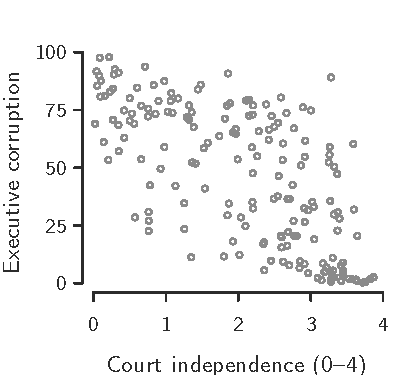
\includegraphics[width=0.95\linewidth]{cd_scatter_1.pdf}
\end{figure}
\onslide<2|handout:0>
\begin{figure}[ht] \centering
        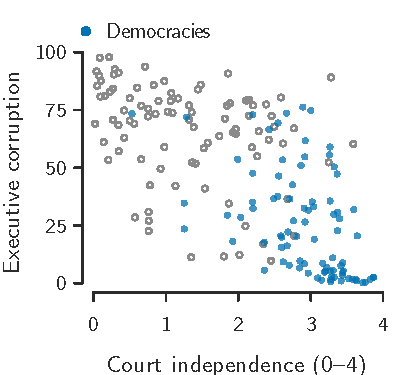
\includegraphics[width=0.95\linewidth]{cd_scatter_2.pdf}
\end{figure}
\onslide<3|handout:0>
\begin{figure}[ht] \centering
        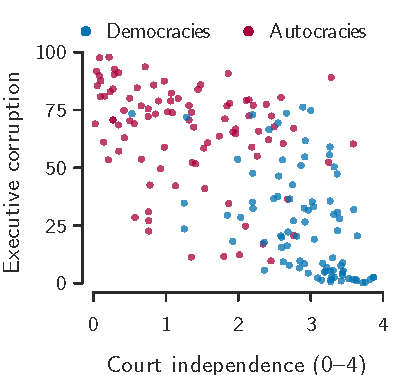
\includegraphics[width=0.95\linewidth]{cd_scatter_3.pdf}
\end{figure}
\onslide<4,5|handout:1>
\begin{figure}[ht] \centering
        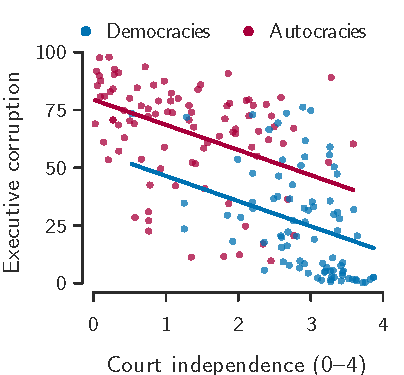
\includegraphics[width=0.95\linewidth]{cd_scatter_4.pdf}
\end{figure}
\end{overprint}

\end{column}
\end{columns}
\slidesource{V-Dem v16, 2024 (executive corruption index $\times$ 100; high court independence).}
}



\frame{
\frametitle{Corruption, Court Independence, and Democracy}
\small
We may want to allow the slopes to differ by including an interaction
term and thereby generalize our regression equation:
\[
Y=\beta_0 + \beta_1 \,X_{court} + \beta_2 \,Z_{dem} + \beta_3 \, (X_{court} \cdot Z_{dem}) + u
\]
%This implies that we want to predict $Y$ using the information we
%have about $X$ and $Z$, but we are no longer assuming an additive
%functional form.
What does this mean?
\pause
When $Z_i = 0$ (autocracies):
\begin{align*}
  \hat Y_i &=\widehat{\beta}_0 + \widehat{\beta}_1 \,X_{court} + \widehat{\beta}_2 \,Z_{dem} + \widehat{\beta}_3 \, (X_{court} \cdot Z_{dem})   \\
  \hat Y_i & = \widehat{\beta}_0 + \widehat{\beta}_1 \,X_{court}
\end{align*}
\pause
When $Z_i = 1$ (democracies):
\begin{align*}
  \hat Y_i &=\widehat{\beta}_0 + \widehat{\beta}_1 \,X_{court} + \widehat{\beta}_2 \,Z_{dem} + \widehat{\beta}_3 \, (X_{court} \cdot Z_{dem})   \\
  \hat Y_i & = (\widehat{\beta}_0 + \widehat{\beta}_2) + (\widehat{\beta}_1+\widehat{\beta}_3) \,X_{court}
\end{align*}
We fit two lines with different slopes AND
different intercepts.
}

\frame{
\frametitle{Corruption, Court Independence, and Democracy}
\begin{columns} [T]
\begin{column}[]{9cm}
\begin{itemize}
\item From R, we obtain estimates $\widehat{\beta}_0,\, \widehat{\beta}_1,\, \widehat{\beta}_2,\, \widehat{\beta}_3$:
\begin{tabular}{c|c|c|c}
%  \hline
  Cons & Court & Dem & Court:Dem \\
  75.3 & $-7.7$ & 2.7 & $-10.3$ \\
\end{tabular}\medskip
\uncover<2->{\item Autocracies:
\begin{align*}
\widehat{y} &= \widehat{\beta}_0 + \widehat{\beta}_1 X_{court}\\
\widehat{y} &= 75.3 - 7.7 \,X_{court}
\end{align*}\vspace{-1em}
}
\uncover<3->{\item Democracies:
\begin{align*}
\widehat{y} &= (\widehat{\beta}_0 + \widehat{\beta}_2) + (\widehat{\beta}_1+\widehat{\beta}_3) \,X_{court}\\
\widehat{y} &= 78.0 - 18.0\, X_{court}
\end{align*}
}
\end{itemize}
\end{column}
\begin{column}[]{6cm}
\begin{overprint}
\onslide<1|handout:0>
\begin{figure}[ht] \centering
        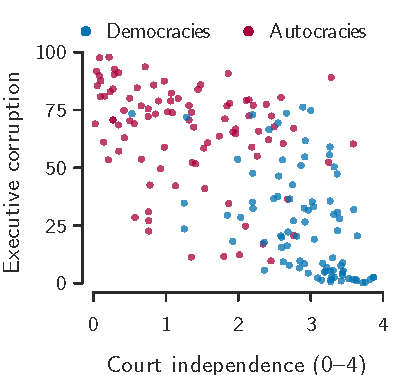
\includegraphics[width=0.95\linewidth]{cd_inter_1.pdf}
\end{figure}
\onslide<2|handout:0>
\begin{figure}[ht] \centering
        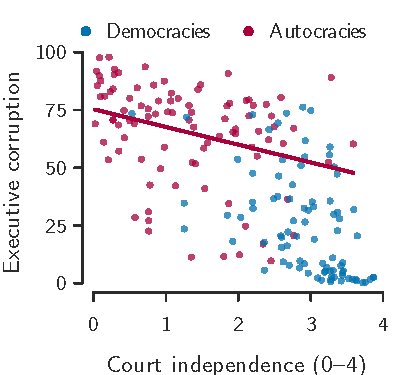
\includegraphics[width=0.95\linewidth]{cd_inter_2.pdf}
\end{figure}
\onslide<3|handout:1>
\begin{figure}[ht] \centering
        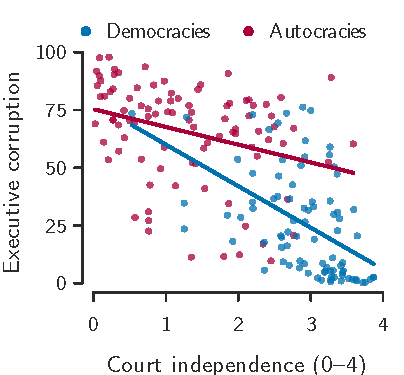
\includegraphics[width=0.95\linewidth]{cd_inter_3.pdf}
\end{figure}
\end{overprint}

\end{column}
\end{columns}
}


\frame{
\frametitle{Corruption, Court Independence, and Democracy}
\begin{columns} [T]
\begin{column}[]{9cm}
\small
Our prediction equation is:\\
$\hat Y_i = 75.3 - 7.7\,X_{court,i} + 2.7\, Z_{dem,i}- 10.3(X_{court,i} \cdot Z_{dem,i})$\\
Where do these quantities appear?
\begin{itemize}
\uncover<2->{\item $\widehat{\beta}_0 = 75.3$ is the
intercept for the prediction
line for autocracies.
}
\uncover<3->{\item $\widehat{\beta}_1 = -7.7$ is the slope for
autocracies.
}
\uncover<4->{\item $\widehat{\beta}_2 = 2.7$ is the vertical
distance between
intercepts, at $X_{court}=0$, where there are no democracies (the least independent court in a democracy scores 0.53).
}
\uncover<5->{\item $\widehat{\beta}_3 =
-10.3$ is the
difference in slopes.}
\end{itemize}
\end{column}
\begin{column}[]{6cm}
\begin{overprint}
\onslide<2|handout:0>
\begin{figure}[ht] \centering
        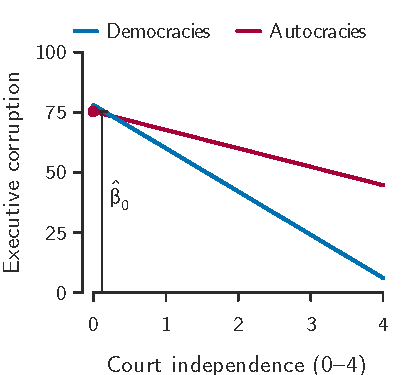
\includegraphics[width=0.95\linewidth]{cd_coef_1.pdf}
\end{figure}
\onslide<3|handout:0>
\begin{figure}[ht] \centering
        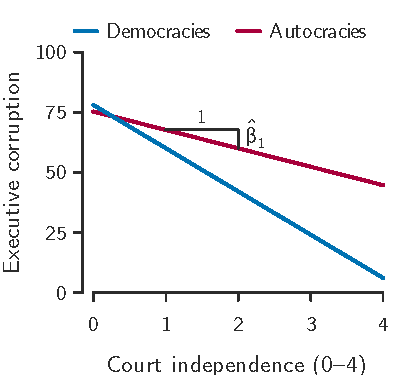
\includegraphics[width=0.95\linewidth]{cd_coef_2.pdf}
\end{figure}
\onslide<4|handout:0>
\begin{figure}[ht] \centering
        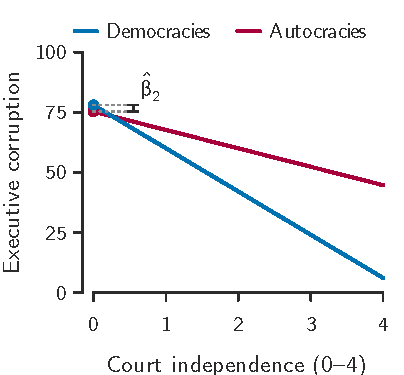
\includegraphics[width=0.95\linewidth]{cd_coef_3.pdf}
\end{figure}
\onslide<5|handout:1>
\begin{figure}[ht] \centering
        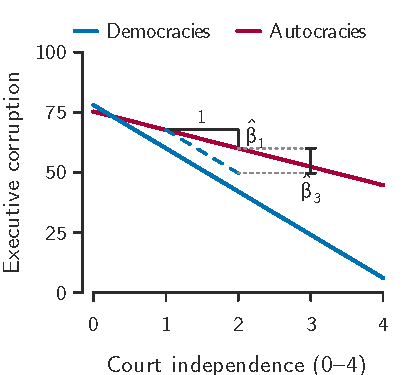
\includegraphics[width=0.95\linewidth]{cd_coef_4.pdf}
\end{figure}
\end{overprint}

\end{column}
\end{columns}
}


\frame{
\frametitle{Corruption, Court Independence, and Democracy}
\begin{columns} [T]
\begin{column}[]{9cm}
\begin{itemize}
\item Again, these observations are
located in three-dimensional
space, which we can view from
different angles.\medskip
\item When we include an interaction
term, the regression surface is
no longer a simple plane; it is twisted
in a certain way.\medskip
\item If we slice through the surface
holding one of the variables
fixed, the slice is still linear.
\end{itemize}
\end{column}
\begin{column}[]{6cm}
\begin{overprint}
\onslide<1|handout:0>
\begin{figure}[ht] \centering
        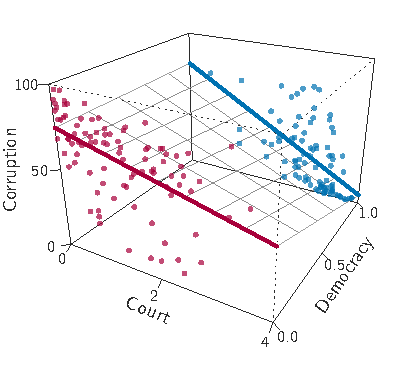
\includegraphics[width=0.95\linewidth]{cd_surface_1.pdf}
\end{figure}
\onslide<2|handout:0>
\begin{figure}[ht] \centering
        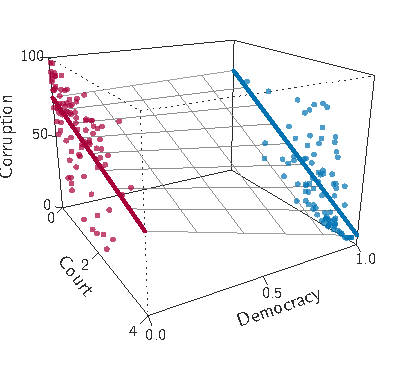
\includegraphics[width=0.95\linewidth]{cd_surface_2.pdf}
\end{figure}
\onslide<3|handout:1>
\begin{figure}[ht] \centering
        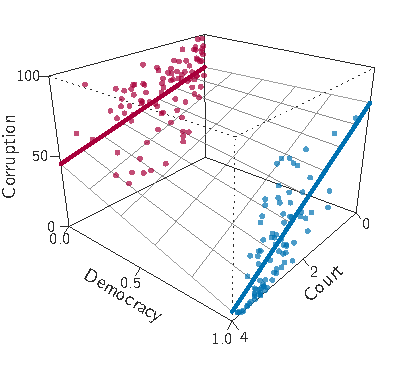
\includegraphics[width=0.95\linewidth]{cd_surface_3.pdf}
\end{figure}
\end{overprint}

\end{column}
\end{columns}
}

\frame{
\frametitle{Do $\hat\beta_{1}$ and $\hat\beta_{2}$ still represent marginal effects?}
\textbf{Worksheet Q1}\medskip

Let $X_{court}$ be high court independence (0--4) and $Z_{dem}\in\{0,1\}$ indicate democracy. Estimate
\[
Y=\beta_0+\beta_1 X_{court}+\beta_2 Z_{dem}+\beta_3(X_{court}\cdot Z_{dem})+u.
\]
\begin{enumerate}\itemsep1em
\item Derive (a) the conditional marginal effect of court independence at regime type $Z=z$ and (b) the conditional marginal effect of democracy at court independence $X=x$.  
\item Using the delta method, give $\mathrm{Var}\!\big(\widehat{\text{ME}}_{court}(z)\big)$ and $\mathrm{Var}\!\big(\widehat{\text{ME}}_{dem}(x)\big)$, where $\widehat{\text{ME}}_{court}(z)=\hat\beta_1+\hat\beta_3 z$ and $\widehat{\text{ME}}_{dem}(x)=\hat\beta_2+\hat\beta_3 x$.  
\item Explain why omitting the covariance term biases the standard errors.  
\end{enumerate}

}

%\frame{
%\frametitle{The Adverse Effects of Sunshine?}
%
%\begin{figure}[ht] \centering
%        \scalebox{.40}{\includegraphics{Malesky3.pdf}}
%\end{figure}
%\tiny{ E. Malesky, P. Schuler and A. Tran (2012). The Adverse Effects of Sunshine: A Field Experiment on Legislative Transparency in an Authoritarian Assembly. \emph{American Political Science Review}, 106, pp 762-786.\\ \bigskip
%
%``The component terms in the interaction are not robustly significant, but are uniformly positively signed. Nevertheless, we cannot say definitively that the transparency or Internet penetration has an independent effect on delegate participation.''}
%
%}




\frame{
\frametitle{Corruption, Court Independence, and Democracy}
To communicate interactions effectively it is often helpful to draw \alert{conditional marginal effect plots} that visualize the marginal effect of one variable at different levels of the other variable.

{\centering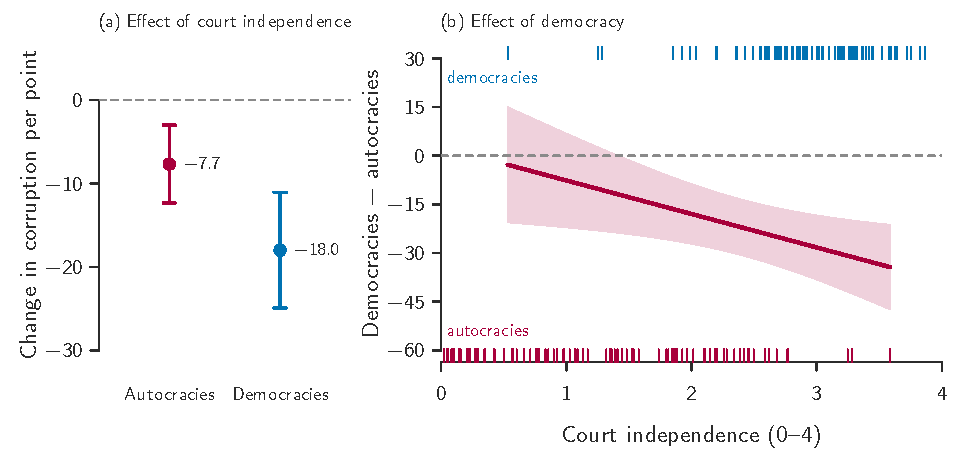
\includegraphics[height=0.56\textheight]{cd_me.pdf}\par}
{\small (a) Independent courts go with less executive corruption in both regime types, and more so in democracies.\\
(b) Drawn only where both groups have data (0.53 to 3.59). The line would cross zero at 0.26, where there are no democracies.}
}


% New frame (2026-10-11, Yiqing): Lecture 5-3 ends by saying its two separate Brexit slopes (1.47 in England
% and Wales, 0.60 in Scotland) are an interaction, the topic of 5-4. This frame takes that up.
% Numbers: code/scotland_interaction.R (output in code/scotland_interaction_output.txt).
\begin{frame}[fragile]
\frametitle{Back to Lecture 5-3: Leave, Scotland, and No Qualifications}
\small
In Lecture 5-3, Leave rose with \texttt{NoQual} (\% of residents aged 16+ with no qualifications, 2011) more steeply in England \& Wales than in Scotland. One interaction model gives both lines:
\spacingset{0.8}
\begin{Verbatim}[fontsize=\footnotesize, frame=single, label=R Code]
> summary(lm(Leave ~ Scotland * NoQual, data = D))
                Estimate Std. Error t value Pr(>|t|)
(Intercept)     21.32652    1.53389  13.904  < 2e-16 ***
Scotland         1.66270    7.22182   0.230  0.81804
NoQual           1.47473    0.06667  22.119  < 2e-16 ***
Scotland:NoQual -0.87536    0.26714  -3.277  0.00115 **
\end{Verbatim}
\spacingset{1}
\begin{itemize}
\item Slope in England \& Wales: 1.47473. Slope in Scotland: $1.47473 - 0.87536 = 0.59937$. These are the two separate lines of Lecture 5-3 (1.47 and 0.60).
\item The interaction tests whether the slopes differ: $t=-3.28$, $p=0.001$.
\item The Scotland coefficient (1.66) is the gap at \texttt{NoQual} $=0$, far below every area (the lowest is 6.7\%).
\end{itemize}
\slidesource{Electoral Commission (2016); 2011 Census (ONS, National Records of Scotland). Data as in Lecture 5-3.}
\end{frame}

\subsection{Interaction between Two Continuous Variables}

\frame{
\frametitle{Interacting continuous variables}

We can generalize to interactions with two continuous variables:
\[
Y=\beta_0 + \beta_1 \,X_1 + \beta_2 \,X_2 + \beta_3 \, (X_1 \cdot X_2) + u
\]

\medskip
What does this imply?\pause
\begin{itemize}
  \item The marginal ``effect'' of $X_1$ is different for each value of $X_2$.
  \item The marginal ``effect'' of $X_2$ is different for each value of $X_1$.
\end{itemize}
}

\frame{
\frametitle{Example: Interacting continuous variables}
\small
Let's illustrate it with the Brexit vote of Lecture 5-3, following Becker, Fetzer \& Novy (2017), ``Who Voted for Brexit?'' \emph{Economic Policy} 32(92): 601--650.\\\medskip

Outcome is the \alert{Leave share} in the 2016 referendum, in the 380 counting areas of Great Britain.\\\medskip
They ask whether the arrival of migrants from Eastern Europe went with a larger Leave vote where more residents had no qualifications.\\\medskip
The variables are defined as follows:
\begin{itemize}
  \item {\tt leave} is Leave as a percentage of valid votes.
  \item {\tt noqual} is the percentage of residents aged 16--74 with no qualifications (or only ``other'' qualifications of unknown level) in 2001, as in Becker et al. (Lecture 5-3 used the 2011 share of residents aged 16+.)
\item {\tt growth} is the growth in residents born in the 12 countries that joined the EU in 2004 and 2007, from 2001 to 2011, as percentage points of the 2001 population. Zero means no net change in that group.
\end{itemize}

}


\frame{
\frametitle{Leave, Qualifications, and Migration}
\begin{columns} [c]
\begin{column}[]{9cm}
\begin{itemize}
\item The bivariate relationship
between Leave and no qualifications is
positive (1.09 points per percentage point).\medskip
\item The bivariate relationship
between Leave and migrant growth is
weak ($-0.64$, $t=-1.9$). Growth is skewed. The median area grew by 1.1 points, Boston by 12.1.\medskip
\item Becker et al.\ ask whether there
is an interaction
between the two variables.
\end{itemize}
\end{column}
\begin{column}[]{6cm}
\begin{overprint}
\onslide<1|handout:0>
\begin{figure}[ht] \centering
        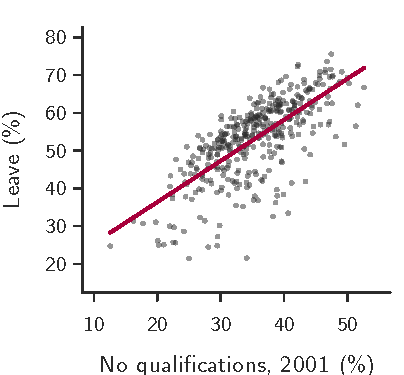
\includegraphics[width=0.95\linewidth]{bx_scatter_1.pdf}
\end{figure}
\onslide<2|handout:1>
\begin{figure}[ht] \centering
        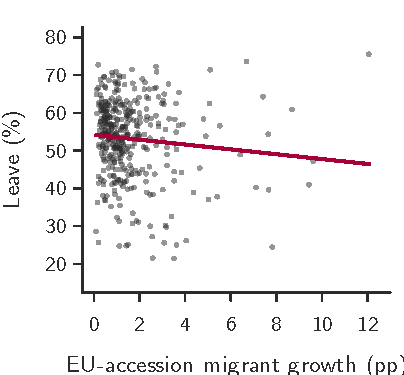
\includegraphics[width=0.95\linewidth]{bx_scatter_2.pdf}
\end{figure}
\end{overprint}

\end{column}
\end{columns}
\slidesource{Electoral Commission (2016); Census 2001 and 2011 (ONS, National Records of Scotland). Design of Becker, Fetzer \& Novy (2017), Table 6.}
}



\frame{
\frametitle{Leave, Qualifications, and Migration}

\begin{columns} [c]
\begin{column}[]{9cm}
\begin{itemize}
\uncover<1->{\item We can plot this data in a
three-dimensional scatterplot.\medskip
}
\uncover<2->{\item When we add in the regression
surface, we see that it is quite
complex...\medskip
}
\uncover<3->{\item ...even when viewed from
different angles.\medskip
}
\uncover<4->{\item or when adding some shading to the surface.
}
\end{itemize}
\end{column}

\begin{column}[]{6cm}
\begin{overprint}
\onslide<1|handout:0>
\begin{figure}[ht] \centering
        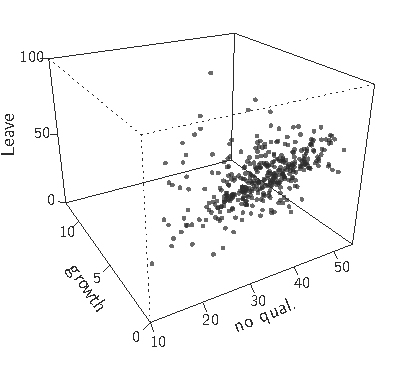
\includegraphics[width=0.95\linewidth]{bx_3d_1.pdf}
\end{figure}
\onslide<2|handout:0>
\begin{figure}[ht] \centering
        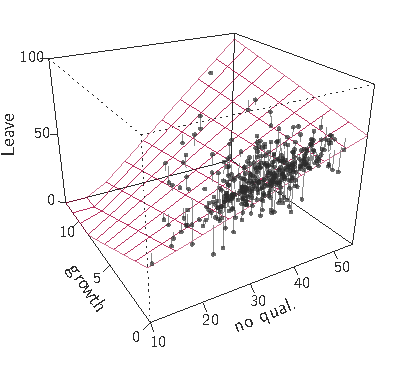
\includegraphics[width=0.95\linewidth]{bx_3d_2.pdf}
\end{figure}
\onslide<3|handout:0>
\begin{figure}[ht] \centering
        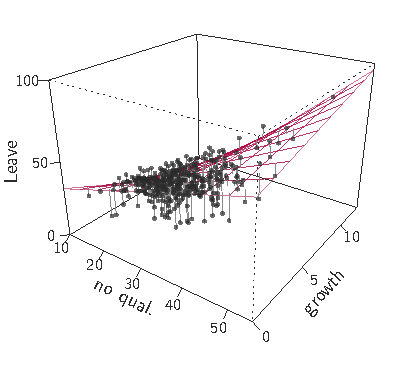
\includegraphics[width=0.95\linewidth]{bx_3d_3.pdf}
\end{figure}
\onslide<4|handout:0>
\begin{figure}[ht] \centering
        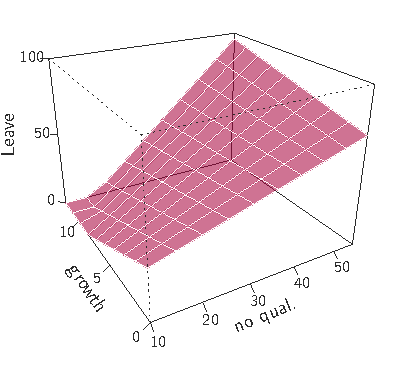
\includegraphics[width=0.95\linewidth]{bx_3d_4.pdf}
\end{figure}
\onslide<5|handout:0>
\begin{figure}[ht] \centering
        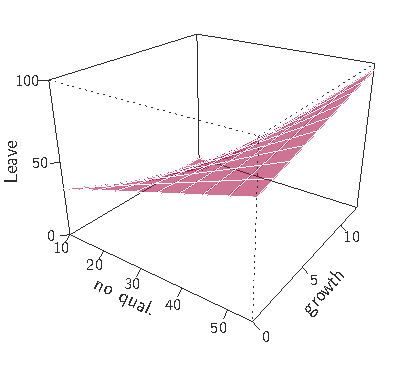
\includegraphics[width=0.95\linewidth]{bx_3d_5.pdf}
\end{figure}
\onslide<6|handout:1>
\begin{figure}[ht] \centering
        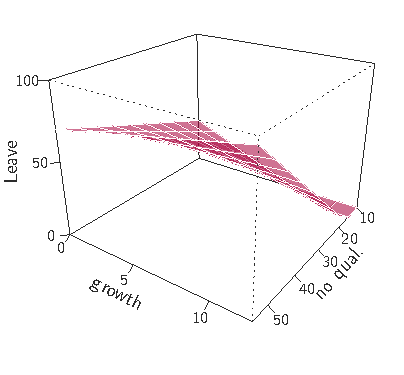
\includegraphics[width=0.95\linewidth]{bx_3d_6.pdf}
\end{figure}
\end{overprint}
\end{column}
\end{columns}
}

\frame{
\frametitle{Leave, Qualifications, and Migration}
\small
\begin{columns} [c]
\begin{column}[]{9cm}
\begin{itemize}
\uncover<1->{\item As before, we can think of this
as defining a regression line for
no qualifications at every level of
migrant growth.
\medskip
}
\uncover<2->{\item The function that describes how $E[Y|X_1,X_2]$ varies with $X_1$ given different levels of $X_2$ is given by:\\
$\widehat{y}_i = (\widehat{\beta}_0+\widehat{\beta}_2 \cdot X_2) +  (\widehat{\beta}_1+\widehat{\beta}_3 \cdot X_2) \cdot X_1$
}
\uncover<3->{\item The conditional marginal effect of $X_1$ given different levels of $X_2$ is:\\
$\frac{\partial \widehat{Y}}{\partial X_1} = \widehat{\beta}_1+\widehat{\beta}_3 \cdot X_2$
%You can use \texttt{lincom}
}
\uncover<4->{\item Here $\widehat{Y} = 24.1 + 0.85\,X_1 - 5.31\,X_2 + 0.133\,X_1X_2$ (robust $t=4.8$ on $X_1X_2$). The slope of no qualifications is 0.85 at zero growth, 0.98 at 1 point, 1.25 at 3, and 1.65 at 6.
}
\end{itemize}
\end{column}
\begin{column}[]{6cm}
\begin{overprint}
\onslide<1|handout:0>
\begin{figure}[ht] \centering
        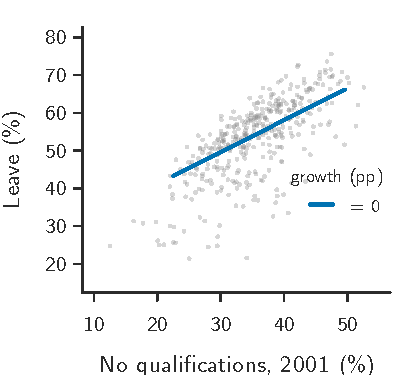
\includegraphics[width=0.95\linewidth]{bx_lines_1.pdf}
\end{figure}
\onslide<2|handout:0>
\begin{figure}[ht] \centering
        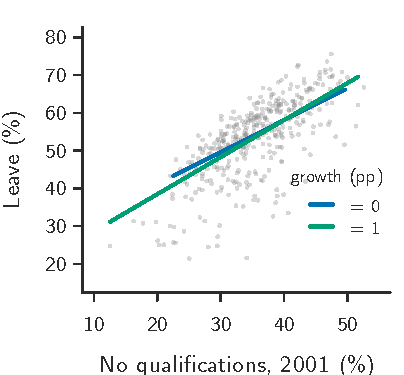
\includegraphics[width=0.95\linewidth]{bx_lines_2.pdf}
\end{figure}
\onslide<3|handout:0>
\begin{figure}[ht] \centering
        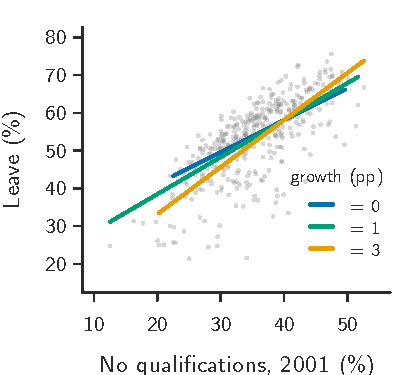
\includegraphics[width=0.95\linewidth]{bx_lines_3.pdf}
\end{figure}
\onslide<4|handout:1>
\begin{figure}[ht] \centering
        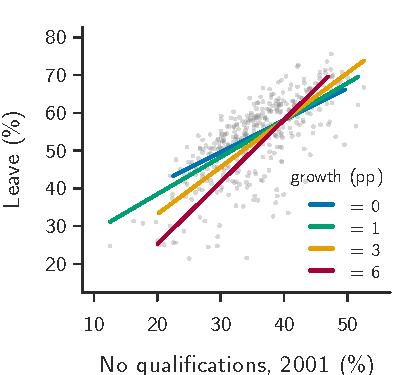
\includegraphics[width=0.95\linewidth]{bx_lines_4.pdf}
\end{figure}
\end{overprint}
\end{column}
\end{columns}
}

\subsection{Interaction Terms: Common Pitfalls and Solutions}

\frame{
\frametitle{Common Pitfalls}
\small
\begin{enumerate}
  \item Omission of lower order/component terms
  \item Misinterpretation of the coefficients on the lower order/component terms as ``direct'' effects
  \item Ignoring the covariance for computation of standard errors of conditional marginal effects
  \item Excessive extrapolation for the conditional effects
  \item False linearity assumptions
\end{enumerate}

\textbf{Read:} Hainmueller, Mummolo, and Xu. 2019. ``How much should we trust estimates from multiplicative interaction models? Simple tools to improve empirical practice.'' \emph{Political Analysis}.
}


\frame{
\frametitle{Omission of lower order terms}

Recall our interaction model
\[
Corruption=\beta_0 + \beta_1 \,Court + \beta_2 \,Dem + \beta_3 \, (Court \cdot Dem) + u
\]
\vspace{-2em}
\begin{columns} [c]
\begin{column}[]{9cm}
\begin{itemize}
\item The fitted line for autocracies:
\begin{align*}
\widehat{y} &= \widehat{\beta}_0 + \widehat{\beta}_1 X_{court}\\
\widehat{y} &= 75.3 - 7.7 \,X_{court}
\end{align*}
\item For democracies:
\begin{align*}
\widehat{y} &= (\widehat{\beta}_0 + \widehat{\beta}_2) + (\widehat{\beta}_1+\widehat{\beta}_3) \,X_{court}\\
\widehat{y} &= 78.0 - 18.0\, X_{court}
\end{align*}
\end{itemize}
\end{column}
\begin{column}[]{6cm}
\begin{figure}[ht] \centering
        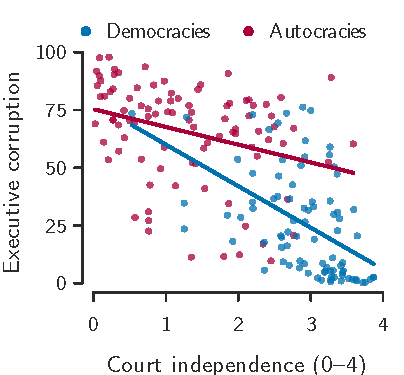
\includegraphics[width=0.95\linewidth]{cd_inter_3.pdf}
\end{figure}
\end{column}
\end{columns}
}


\frame{
\frametitle{Omission of lower order terms}
Suppose we instead omit the lower order term for democracy and fit \\
\[
Corruption=\beta_0 + \beta_1 \,Court + \beta_3 \, (Court \cdot Dem) + u
\]
Q. What do we assume?
\begin{enumerate}
  \item The predicted corruption level is the same in all democracies.
  \item The predicted corruption level is the same in all autocracies.
  \item The slope of the regression line is the same in democracies
and autocracies.
  \item The intercept of the regression line is the same in
democracies and autocracies.
\end{enumerate}
}

\frame{
\frametitle{Omission of lower order terms}
\begin{columns} [c]
\begin{column}[]{9cm}
\begin{itemize}
\item This model implies the following
regression lines for democracies and autocracies.\medskip
\item For autocracies:\\
$Corr. =\beta_0 + \beta_1 \,Court$
\medskip
\item  For democracies:\\
$Corr. =\beta_0 + (\beta_1 + \beta_3) \, Court$
\item Both lines must start from the same point at $Court=0$. The fit hardly changes here (the full model's $\widehat{\beta}_2 = 2.7$), but the interaction's standard error falls from 4.2 to 1.7 ($t$ from $-2.4$ to $-5.6$). The restriction makes the evidence look much stronger than it is.
\item In general, it is a bad idea to fit models that don't include all the
lower order terms. These models impose strict and usually
unrealistic assumptions.
\end{itemize}
\end{column}
\begin{column}[]{6cm}
\begin{overprint}
\onslide<1>
\begin{figure}[ht] \centering
        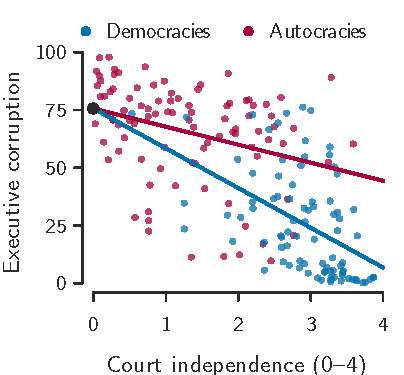
\includegraphics[width=0.95\linewidth]{cd_nomain.pdf}
\end{figure}

\end{overprint}

\end{column}
\end{columns}
}

\frame{
\frametitle{Omission of lower order terms}
Recall the interaction model with two continuous variables $X_1$ and $X_2$:
\[
Y=\beta_0 + \beta_1 \,X_1 + \beta_2 \,X_2 + \beta_3 \, (X_1 \cdot X_2) + u
\]
How do we interpret $\beta_1$ and $\beta_2$? \pause Marginal effects of $X_1$ and $X_2$ when the other variable is zero. In the Brexit model, $\widehat{\beta}_1=0.85$ is the slope of no qualifications where migrant growth is zero, near many real areas (the lowest growth is 0.1). $\widehat{\beta}_2=-5.3$ is the slope of migrant growth where no one lacks qualifications. No area comes close (the lowest share is 12.6\%).\\\medskip

Is it a good idea to omit lower order terms as in?
\[
Y=\beta_0 + \beta_1 \,X_1 + \beta_3 \, (X_1 \cdot X_2) + u
\]
}


\frame{
\frametitle{Omission of lower order terms}
\[
Y=\beta_0 + \beta_1 \,X_1 + \beta_3 \, (X_1 \cdot X_2) + u
\]
As before, it makes no sense to drop lower order terms from the interaction model:
\begin{itemize}
 \item E.g., dropping no qualifications constrains its slope to be zero where migrant growth is zero.
  \item E.g., dropping migrant growth constrains its slope to be zero where no one lacks qualifications.
\item In the Brexit data, dropping migrant growth changes the interaction from 0.13 ($t=4.8$) to $-0.005$ ($t=-0.65$).
\item \alert{Never omit the lower order terms!!!}
\begin{itemize}\small\itemsep0.5em
\item Principle extends to higher order interactions (e.g. for three-way interactions you need to include all three main effects $X_1, X_2, \mbox{ and } X_3$, all two-way interaction terms ($X_1 \cdot X_2$,  $X_1 \cdot X_3$, and $X_2 \cdot X_3$), and the three-way interaction term ($X_1 \cdot X_2 \cdot X_3$))
\item Lower order terms might only be omitted in special cases (e.g. when the lower order term is absorbed in the fixed effects)
\end{itemize}
\end{itemize}
}


\frame{
\frametitle{Misinterpretation of the coefficients on the lower terms}
\small

Recall our interaction model:

$$
Y = \beta_0 +\,\, \beta_1 \,X_{1} +\,\, \beta_2 \, X_{2} + \,\,\beta_3 (X_{1} \cdot X_{2}) + u
$$\\\bigskip
The conditional marginal effect of $X_1$ is therefore conditional on the level of $X_2$:
$$
\frac{\partial Y}{\partial X_{1}} = \beta_{1}+\beta_{3}\cdot X_{2}
$$
Therefore, $\beta_{1}$ is simply the marginal effect of $X_1$ at the point where $X_2=0$. Often, this is not a meaningful quantity of interest because $X_2$ might never take on the value of zero.\\\bigskip

\alert{Never interpret the lower term coefficients $\beta_{1}$ or $\beta_2$ as ``unconditional'', ``direct'', or ``independent'' marginal effects of $X_{1}$ or $X_2$!}
}


\frame{
\frametitle{The Adverse Effects of Sunshine?}

% Table 5 (panel A) of Malesky, Schuler & Tran (2012), typeset from the
% published table; it replaces the unreadable page image Malesky3.pdf.
\begin{center}
\scriptsize
\renewcommand{\arraystretch}{1.1}
\setlength{\tabcolsep}{4pt}
\begin{tabular}{l*{8}{c}}
\hline
 & \multicolumn{4}{c}{Question count (\#)} & \multicolumn{4}{c}{Critical questions (\%)} \\
 & (1) & (2) & (3) & (4) & (5) & (6) & (7) & (8) \\
\hline
Treated & 0.016 & 0.247$^{*}$ & 0.249 & 0.271$^{*}$ & 0.942 & 3.188 & 3.013 & 2.799 \\
 & (0.146) & (0.147) & (0.151) & (0.154) & (1.802) & (2.008) & (1.956) & (1.907) \\
Internet penetration & & 0.058 & 0.062$^{*}$ & 0.105 & & 0.744 & 0.771 & 2.850$^{***}$ \\
 & & (0.035) & (0.033) & (0.070) & & (0.578) & (0.593) & (0.843) \\
Treated $\times$ Internet & & $-$0.170$^{***}$ & $-$0.171$^{***}$ & $-$0.179$^{***}$ & & $-$1.673$^{***}$ & $-$1.658$^{***}$ & $-$1.865$^{***}$ \\
 & & (0.030) & (0.027) & (0.027) & & (0.383) & (0.381) & (0.330) \\
\hline
Individual controls & & & \checkmark & \checkmark & & & \checkmark & \checkmark \\
Provincial controls & & & & \checkmark & & & & \checkmark \\
Observations & 461 & 461 & 461 & 461 & 461 & 461 & 461 & 461 \\
\hline
\end{tabular}

\smallskip
{\small Table 5, panel A: change between Session 5 (Nov.\ 2009) and Session 6 (June 2010). OLS, standard errors clustered by province in parentheses. $^{*}p<.1$, $^{**}p<.05$, $^{***}p<.01$.}
\end{center}
{\small E. Malesky, P. Schuler and A. Tran (2012). The Adverse Effects of Sunshine: A Field Experiment on Legislative Transparency in an Authoritarian Assembly. \emph{American Political Science Review}, 106, pp 762-786.\\ \bigskip

``The component terms in the interaction are not robustly significant, but are uniformly positively signed. Nevertheless, we cannot say definitively that the transparency or Internet penetration has an independent effect on delegate participation.''}

}

\frame{
\frametitle{Ignoring the covariance for variance of conditional effects}
\small

Recall our interaction model:
$$
Y = \beta_0 +\,\, \beta_1 \,X_{1} +\,\, \beta_2 \, X_{2} + \,\,\beta_3 (X_{1} \cdot X_{2}) + u
$$\\\bigskip
The marginal effect of $X_1$ is therefore conditional on the level of $X_2$:
$$
\frac{\partial\hat Y}{\partial X_{1}} = \hat\beta_{1}+\hat\beta_{3}\cdot X_{2}
$$
The variance for the conditional effect of $X_1$ is therefore:
$$
Var \left[ \frac{\partial \hat Y}{\partial X_{1}} \right] = Var[ \hat\beta_{1}+ \hat\beta_{3}\cdot X_{2}] = Var[\hat\beta_1] + X_{2}^2 Var[\hat\beta_3] + 2 X_2 Cov[\hat\beta_{1},\hat\beta_{3}]
$$
\alert{Never forget to include the covariance in computing the variance of the conditional effect }

}

\frame{
\frametitle{Corruption, Court Independence, and Democracy}

{\centering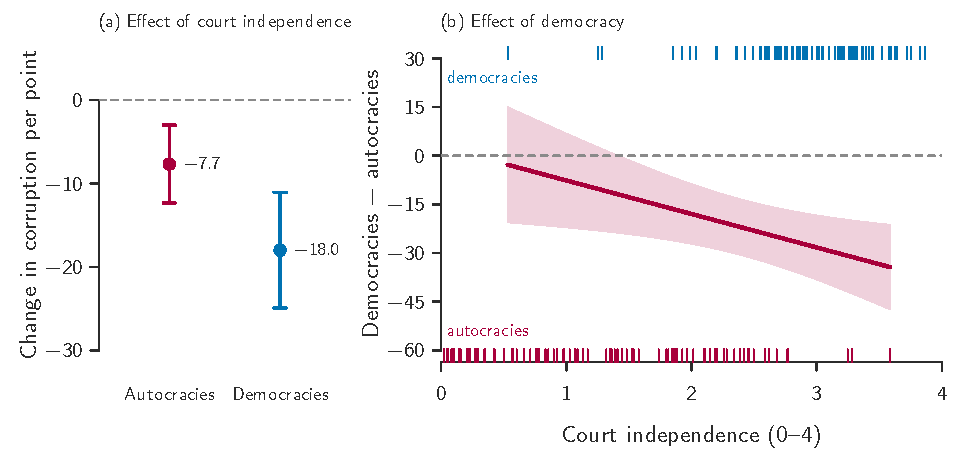
\includegraphics[height=0.82\textheight]{cd_me.pdf}\par}
}

\frame{
\frametitle{Excessive extrapolation for the conditional effects}
\small

Recall our interaction model:

$$
Y = \beta_0 +\,\, \beta_1 \,X_{1} +\,\, \beta_2 \, X_{2} + \,\,\beta_3 (X_{1} \cdot X_{2}) + u
$$\\\bigskip
The marginal effect of $X_1$ is therefore conditional on the level of $X_2$:
$$
\frac{\partial \hat Y}{\partial X_{1}} = \hat\beta_{1}+ \hat\beta_{3}\cdot X_{2}
$$
Need to be careful to only compute this conditional effect for realistic values of $X_2$ (e.g. at the 25th, 50th, and 75th percentile of $X_2$). Computing the effect at levels of $X_2$ where there are no or only few observations requires excessive extrapolation and results in high model dependency.

\medskip

\alert{Never compute the conditional effect of the variable of interest at unrealistic or atypical  values of the conditioning variable. Always show the distribution of the conditioning variable in the plot (e.g. using a rugplot).}

}


\frame{
\frametitle{The Adverse Effects of Sunshine?}

{\small E. Malesky, P. Schuler and A. Tran (2012). The Adverse Effects of Sunshine: A Field Experiment on Legislative Transparency in an Authoritarian Assembly. \emph{American Political Science Review}, 106, pp 762-786.\\ \bigskip

An online newspaper, VietnamNet, reported the legislative activity of a randomly chosen group of delegates to Vietnam's National Assembly. Their Figure 1 plots the estimated effect of this treatment on questions asked and on criticism against Internet subscribers per 100 citizens in the delegate's province: near zero where few people are online, increasingly negative where more are.\\ \bigskip

``We find no evidence of a direct effect of the transparency treatment on delegate performance; however, further analysis reveals that delegates subjected to high treatment intensity demonstrate robust evidence of curtailed participation and damaged reelection prospects. These results make us cautious about the export of transparency without electoral sanctioning.''}

}

\frame{
\frametitle{The Adverse Effects of Sunshine?}
\vspace{-.1in}
\begin{figure}[ht] \centering
        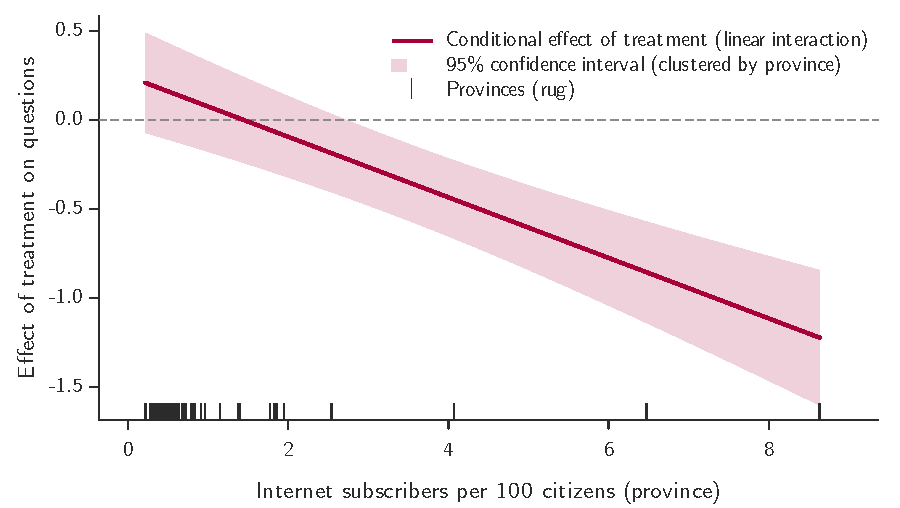
\includegraphics[height=0.64\textheight]{malesky_me_linear.pdf}
\end{figure}
\tiny{ J. Anderson (2013). Sunshine Works. Comment on ``The Adverse Effects of Sunshine: A Field Experiment on Legislative Transparency in an Authoritarian Assembly.'' \emph{World Bank Policy Research Working Paper} 6602.\\\medskip

On the change in \emph{critical} questions: ``there are only three provinces (Hanoi, HCMC, and Da Nang) out of 64 (i.e., fewer than 5 percent of provinces) for which the predicted effect of treatment is statistically significantly different from zero at any conventional level.''}
}

\frame{
\frametitle{The Adverse Effects of Sunshine?}
\vspace{-.1in}
\begin{figure}[ht] \centering
        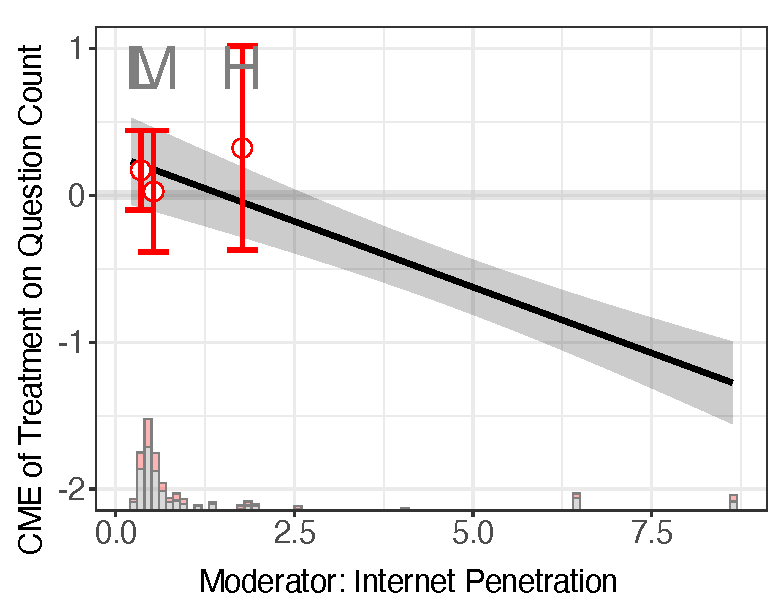
\includegraphics[height=0.72\textheight]{hmx_malesky_bin.pdf}
\end{figure}
\slidesource{Replicates Hainmueller, Mummolo \& Xu (2019), \emph{Political Analysis} 27(2), Figure 6(b).}
}

\frame{
\frametitle{The Adverse Effects of Sunshine?}
\vspace{-.1in}
\begin{figure}[ht] \centering
        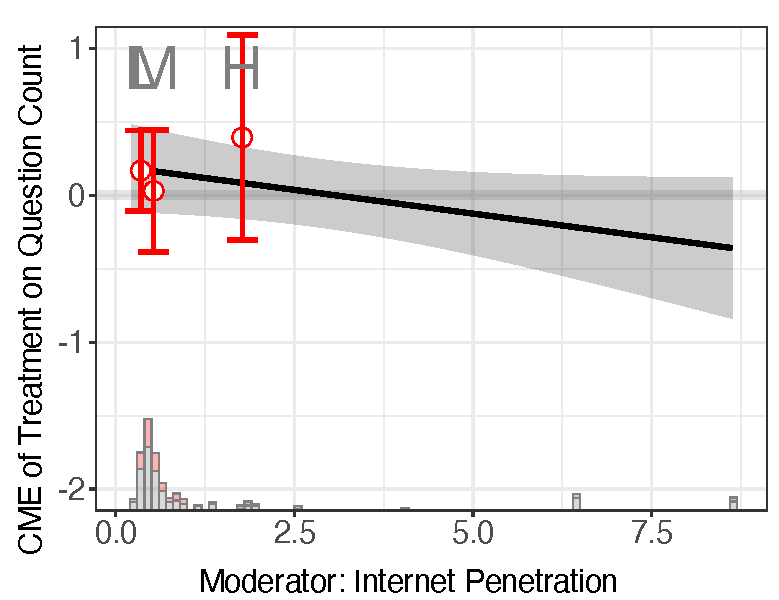
\includegraphics[height=0.72\textheight]{hmx_malesky_bin4.pdf}
\end{figure}
\slidesource{Replicates Hainmueller, Mummolo \& Xu (2019), \emph{Political Analysis} 27(2), Figure 6(c), after dropping four high-leverage delegates.}
}

\frame{
\frametitle{Excessive extrapolation for the conditional effects}
\small

Recall our interaction model:

$$
Y = \beta_0 +\,\, \beta_1 \,X_{1} +\,\, \beta_2 \, X_{2} + \,\,\beta_3 (X_{1} \cdot X_{2}) + u
$$\\\bigskip
The marginal effect of $X_1$ is therefore conditional on the level of $X_2$:
$$
\frac{\partial\hat Y}{\partial X_{1}} = \hat\beta_{1}+\hat\beta_{3}\cdot X_{2}
$$

Another issue you need to check when computing the conditional effect of $X_1$ is whether at the realistic values of $X_2$ there is actually sufficient variation in $X_1$. Computing the effect at levels of $X_2$ where there is no or little variation in $X_1$ requires excessive extrapolation and results in high model dependency.

\bigskip

\alert{Never compute the conditional effect of the variable of interest at values of the conditioning variable where there is no or almost no variation on the variable of interest. Always check the distribution of the variable of interest across the values of the conditioning variable for which you plot the effect.}

}

\frame{
\frametitle{Audience Beliefs and IO Legitimacy?}
\vspace{-.1in}
\begin{figure}[ht] \centering
        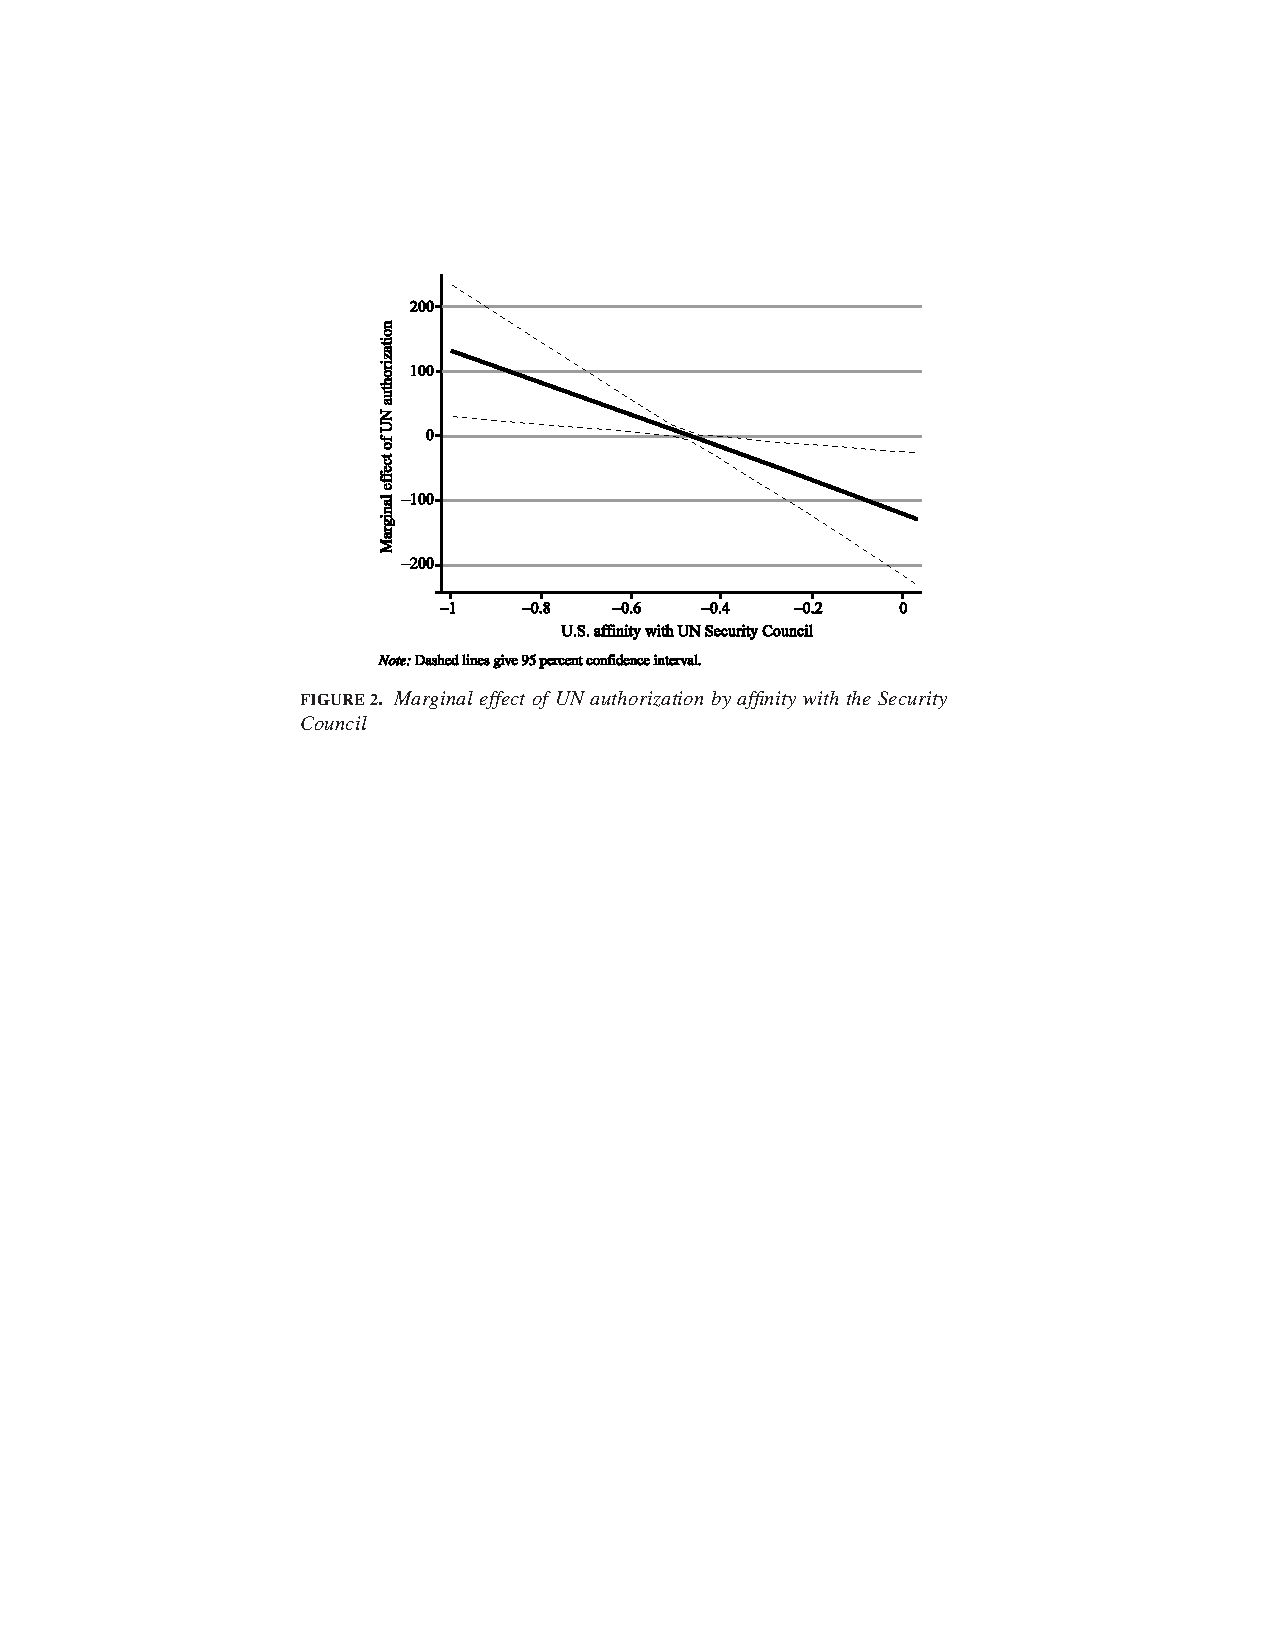
\includegraphics[width=0.53\linewidth]{chap.pdf}
\end{figure}
\tiny{ Chapman,  T. 2009. Audience Beliefs and International Organization Legitimacy. \emph{International Organization}. 63(4):733-764.\\\medskip

Looks at the effect of UN Security Council authorization for use of force on changes in presidential approval (``rallies'') after military onset and how this effect depends on the similarity of preferences between the U.S. and the UN Security Council.\\\medskip

``Clearly, the effect of authorization on rallies decreases as similarity increases.''}
}

\frame{
\frametitle{Audience Beliefs and IO Legitimacy?}
\begin{figure}[ht] \centering
        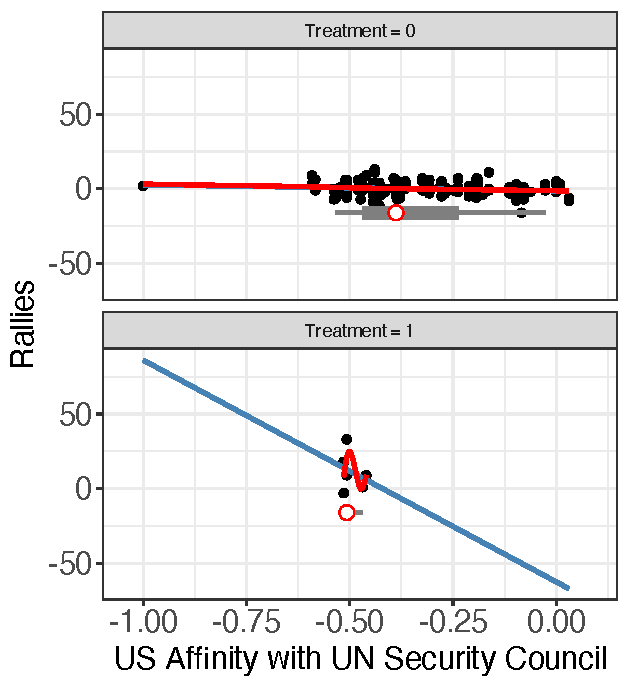
\includegraphics[height=0.72\textheight]{hmx_chapman_raw}
\end{figure}
\slidesource{Replicates Hainmueller, Mummolo \& Xu (2019), \emph{Political Analysis} 27(2), Figure 5(a).}
}

\frame{
\frametitle{Audience Beliefs and IO Legitimacy?}
\begin{figure}[ht] \centering
        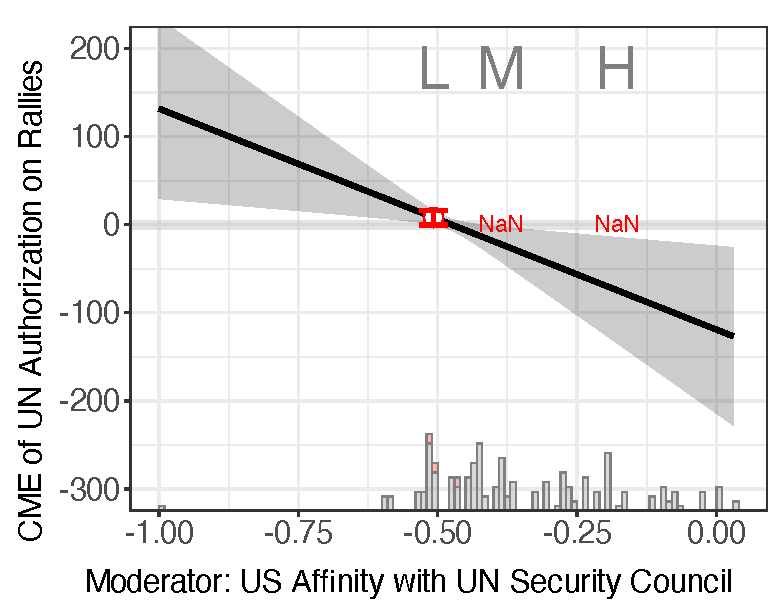
\includegraphics[height=0.72\textheight]{hmx_chapman_bin}
\end{figure}
\slidesource{Replicates Hainmueller, Mummolo \& Xu (2019), \emph{Political Analysis} 27(2), Figure 5(b).}
}

%\frame{
%\frametitle{Audience Beliefs and IO Legitimacy?}
%
%
%
%\begin{figure}[ht] \centering
%        \scalebox{.42}{\includegraphics{chapman_2009_raw.pdf}}
%\end{figure}
%%\tiny{ J. Anderson(2013). Sunshine Works. Comment on The Adverse Effects of Sunshine: A Field Experiment on Legislative Transparency in an Authoritarian Assembly? \emph{Policy Research Working Paper}, 16602.\\ \bigskip
%%
%%``there are only three provinces (Hanoi, HCMC, and Da Nang) out of 64 (i.e., fewer than 5 percent of provinces) for which the predicted effect of treatment is statistically significantly different from zero at any conventional level.''}
%}

\frame{
\frametitle{False linearity assumption}
\small

Recall our interaction model:
$$
Y = \beta_0 +\,\, \beta_1 \,X_{1} +\,\, \beta_2 \, X_{2} + \,\,\beta_3 (X_{1} \cdot X_{2}) + u
$$\\\bigskip
The marginal effect of $X_1$ is therefore conditional on the level of $X_2$:
$$
\frac{\partial Y}{\partial X_{1}} = \beta_{1}+\beta_{3}\cdot X_{2}
$$
The functional form here assumes that the interaction effect is linear, i.e. the marginal effect of $X_1$ changes linearly with levels of $X_2$. But this linearity assumption is often flawed. For example,  the effect of $X_1$ might be large at low levels of $X_2$, small at medium levels of $X_2$, and large at high levels of $X_2$.\\\bigskip

\alert{Always check the linearity assumption by running a more flexible model that allows the conditional effect to vary more freely across levels of the conditioning variable. }

}

\frame{
\frametitle{Relaxing the Linearity Assumption}
\small

%A more flexible model that allows the conditional effect to vary more freely across levels of the conditioning variable

Discretize the conditioning variable $X_2$ into three equal sized bins using three dummy variables $G_{j}$ with $j=1,2,3$:
\[
G_{i1}=\begin{cases}
1 & X_{2i}< \delta_{1/3}\\
0 & otherwise \\
\end{cases},\quad
G_{i2}=\begin{cases}
1 & X_{2i}\in [\delta_{1/3},\delta_{2/3})\\
0 & otherwise
\end{cases},\quad
G_{i3}=\begin{cases}
1 & X_{2i}\geq \delta_{2/3}\\
0 & otherwise
\end{cases},
\]
in which $\delta_{1/3}$ and $\delta_{2/3}$ are respectively the first and second tertiles of $X_2$.\\\medskip
Let $\bar{x}_{1}$, $\bar{x}_{2}$, and $\bar{x}_{3}$ be the median values of $X_2$ in each of the three bins, respectively. \\\medskip

We then estimate the following model:

\begin{equation}\nonumber
Y  = \sum_{j=1}^{3} \{ \mu_{j} + \eta_{j}
(X_2-\bar{x}_{j}) + \alpha_{j} X_1 +
\lambda_{j}(X_2-\bar{x}_{j}) X_1 \}  G_{j} + u
\end{equation}
where $\alpha_{j}$ is the conditional effect of $X_1$ at the bin median $X_2=\bar{x}_{j}$.

}

%To test the assumption of linear marginal effects, Let $x_{1}$, $x_{2}$, and $x_{3}$ be the median
%values of $X$ in each of the three bins, respectively (they can
%virtually be any values within the three intervals).  %

% Frames 42-44 (handout pages): figure in a 0.56 column (just wider than the figure, so no gap before the text), two bullets beside it (Yiqing, 2026-10-11).
% Figures and numbers: code/fig_hmx_interflex.R (interflex dev branch; same estimates as CRAN 1.4.1).
\frame{
\frametitle{The Adverse Effects of Sunshine?}
\begin{columns}[c,onlytextwidth]
\begin{column}{0.56\textwidth}
        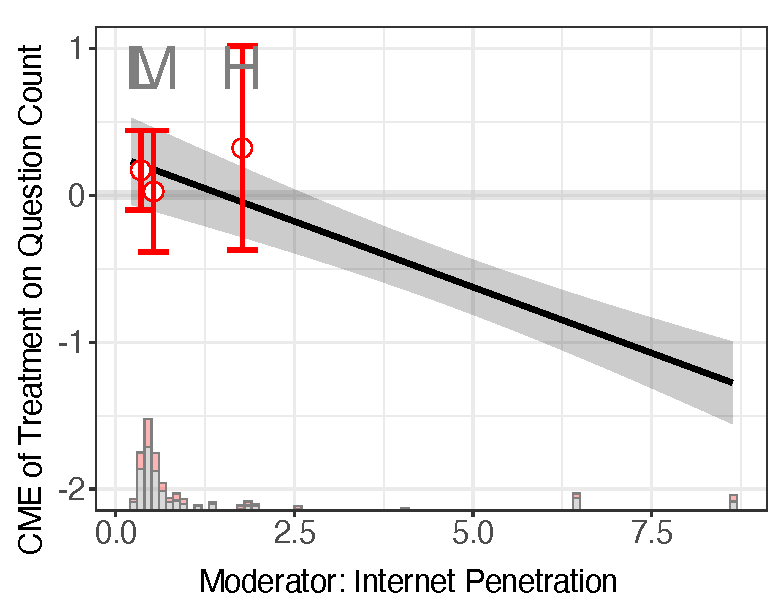
\includegraphics[width=\linewidth]{hmx_malesky_bin.pdf}
\end{column}
\begin{column}{0.42\textwidth}
\small\setlength{\leftmargini}{1.1em}
\begin{itemize}\itemsep1em
\item The bin estimates at low, medium and high Internet penetration are 0.17, 0.03 and 0.32. None differs from zero at the 5\% level.
\item The bin estimates do not fall as the line does. The line's large negative effects lie where the histogram shows almost no delegates.
\end{itemize}
\end{column}
\end{columns}
\slidesource{Malesky, Schuler \& Tran (2012) data, with their covariates; SEs clustered by province. Replicates Hainmueller, Mummolo \& Xu (2019), Figure 6(b).}
}

\frame{
\frametitle{Linear Interaction? Clark and Golder (2006)}
\begin{columns}[c,onlytextwidth]
\begin{column}{0.56\textwidth}
        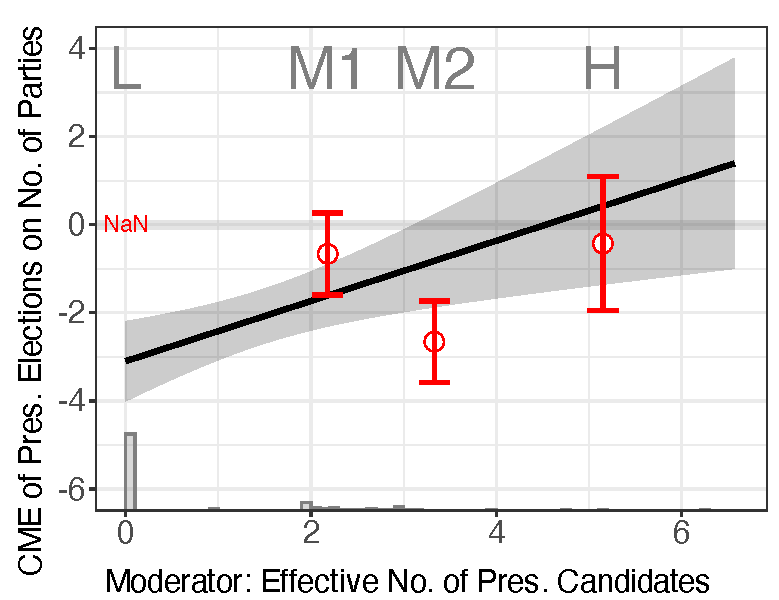
\includegraphics[width=\linewidth]{hmx_clark_bin.pdf}
\end{column}
\begin{column}{0.42\textwidth}
\small\setlength{\leftmargini}{1.1em}
\begin{itemize}\itemsep1em
\item Bin L has no estimate. With no presidential election ($X=0$), the treatment is always 0.
\item The effect is $-2.66$ at M2, far below the line, and its interval excludes zero. At M1 and H it is near zero. The effect does not change linearly with $X$.
\end{itemize}
\end{column}
\end{columns}
\slidesource{Clark \& Golder (2006) data; SEs clustered by country. Replicates Hainmueller, Mummolo \& Xu (2019), Figure 7(a).}
}

\frame{
\frametitle{Linear Interaction! Huddy et al (2015)}
\begin{columns}[c,onlytextwidth]
\begin{column}{0.56\textwidth}
        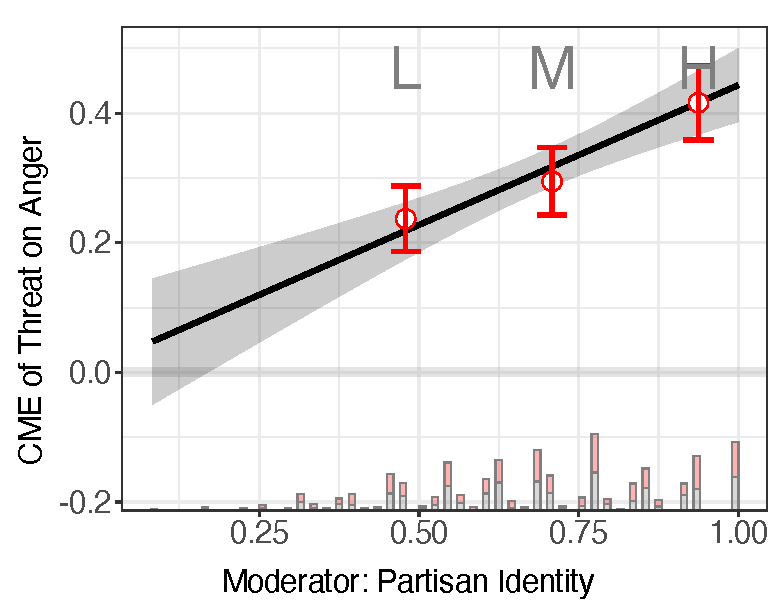
\includegraphics[width=\linewidth]{hmx_huddy_bin.pdf}
\end{column}
\begin{column}{0.42\textwidth}
\small\setlength{\leftmargini}{1.1em}
\begin{itemize}\itemsep1em
\item The bin estimates rise with partisan identity, from 0.24 to 0.29 to 0.42. Each differs from zero.
\item Each is close to the line. Here the linear interaction model holds up.
\end{itemize}
\end{column}
\end{columns}
\slidesource{Huddy, Mason \& Aar{\o}e (2015) data; robust SEs. Replicates Hainmueller, Mummolo \& Xu (2019), Figure 4(b).}
}

% Three frames added 2026-10-10 (Yiqing: explain better how the interflex kernel estimator works, then mention
% the DML extension in the new interflex; since 2026-10-11 only a mention, as DML is taught in 450B). Figure and numbers: code/fig_kernel_court.R (interflex 1.4.1; v2 2026-10-11: running example, court independence x democracy).
\frame{
\frametitle{A More Flexible Estimator: The Kernel Estimator}
\small
Binning estimates the effect at three points. The \alert{kernel estimator} (Hainmueller, Mummolo \& Xu 2019, Section 4.2) estimates it across the whole range of $X$ in the model
\[
Y = f(X) + g(X)\,D + \gamma(X)\,Z + \epsilon,
\]
where $f$, $g$ and $\gamma$ are smooth functions of $X$ and $g(X)$ is the conditional marginal effect of $D$. The linear interaction model is the special case $f(X)=\mu+\eta X$, $g(X)=\alpha+\beta X$, $\gamma(X)=\gamma$.\medskip

For each evaluation point $x_0$, fit the interaction model \alert{locally}, by weighted least squares:
\[
\min_{\mu,\alpha,\eta,\beta,\gamma}\ \sum_{i=1}^{N} \big[Y_i-\mu-\alpha D_i-\eta(X_i-x_0)-\beta D_i(X_i-x_0)-\gamma Z_i\big]^2\, K\!\Big(\frac{X_i-x_0}{h}\Big),
\]
and set $\hat g(x_0)=\hat\alpha(x_0)$. Repeating this over a grid of $x_0$ traces out $\hat g(\cdot)$.
\begin{itemize}
\item $K$ is a Gaussian kernel: units with $X_i$ near $x_0$ get the most weight.
\item The bandwidth $h$ is chosen by cross-validation; \texttt{interflex} makes it wider where the data on $X$ are sparse.
\item Confidence intervals come from the bootstrap (a block bootstrap with clusters).
\item Newer versions of \texttt{interflex} also offer double/debiased machine learning (DML) estimators (Liu, Liu \& Xu 2025), covered in 450B.
\end{itemize}
}

\frame{
\frametitle{Audience Beliefs and IO Legitimacy?}
\begin{figure}[ht] \centering
        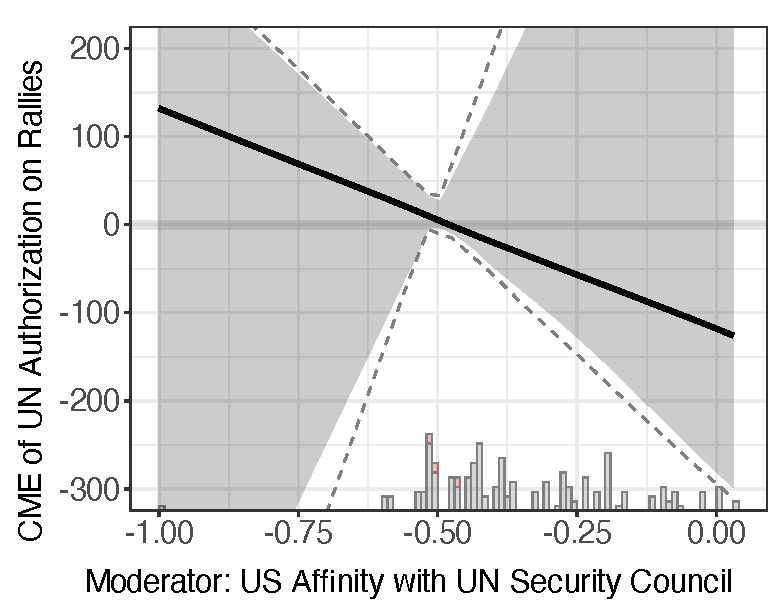
\includegraphics[height=0.72\textheight]{hmx_chapman_kernel}
\end{figure}
\slidesource{Replicates Hainmueller, Mummolo \& Xu (2019), \emph{Political Analysis} 27(2), Figure 5(c), bandwidth by cross-validation (0.34; their code: 0.30).}
}

\frame{
\frametitle{Kernel Estimator: Corruption, Courts, and Democracy}
\begin{columns}[c,onlytextwidth]
\begin{column}{0.66\textwidth}
        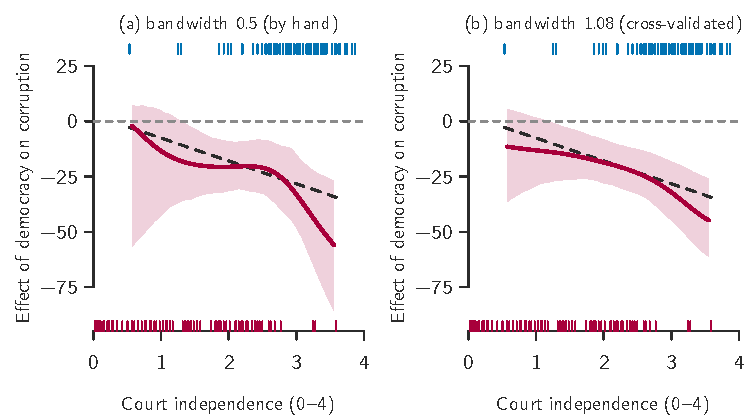
\includegraphics[width=\linewidth]{kernel_court.pdf}\par\smallskip
{\footnotesize Effect of democracy ($D$) on executive corruption across court independence ($X$), with pointwise 95\% bootstrap intervals (500 resamples), drawn where both groups have data. Dashed: the linear interaction model. Ticks: autocracies (bottom), democracies (top).}
\end{column}
\begin{column}{0.32\textwidth}
\small\setlength{\leftmargini}{1.1em}
\begin{itemize}\itemsep1em
\item With $h = 0.5$ the effect stays near $-20$ from court independence 1.4 to 2.5, then drops past 2.8, where only three autocracies sit. The interval is wide at both ends.
\item Cross-validation picks $h=1.08$, whose curve stays close to the line. Every $h$ from about 0.4 up fits about as well (loss 8.54 at $h=0.49$, 8.46 at 1.08, 8.53 at 3.84; SE 0.78). The kernel estimates do not contradict the linear model here.
\end{itemize}
\end{column}
\end{columns}
\slidesource{V-Dem v16, 2024.}
}

% DML frame cut 2026-10-11 (Yiqing: DML is taught in 450B; a mention on the kernel slide is enough).

%\tiny{ J. Anderson(2013). Sunshine Works. Comment on The Adverse Effects of Sunshine: A Field Experiment on Legislative Transparency in an Authoritarian Assembly? \emph{Policy Research Working Paper}, 16602.\\\medskip
%
%``there are only three provinces (Hanoi, HCMC, and Da Nang) out of 64 (i.e., fewer than 5 percent of provinces) for which the predicted effect of treatment is statistically significantly different from zero at any conventional level.''}


\frame{
\frametitle{How Much Should We Trust Linear Interaction Models?}
% Table 1 of Hainmueller, Mummolo & Xu (2019), typeset; it replaces the
% screenshot figX.pdf.
\begin{center}
\small
\renewcommand{\arraystretch}{1.3}
\begin{tabular}{lccccc}
\hline
 & & Not rejecting & Severe & Rejecting & Mean \\
Journal & $N$ & same effect at low vs.\ high & extrapolation & linear model & score \\
\hline
AJPS & 9 & 0.78 & 0.78 & 0.22 & 1.8 \\
APSR & 17 & 0.71 & 0.41 & 0.65 & 1.8 \\
CPS & 10 & 0.67 & 0.3 & 0.5 & 1.3 \\
IO & 7 & 0.83 & 0.71 & 0.67 & 2.3 \\
JOP & 3 & 0.33 & 0.33 & 0.67 & 1.3 \\
\hline
All journals & 46 & 0.71 & 0.50 & 0.52 & 1.7 \\
\hline
\end{tabular}
\end{center}

\medskip
{\footnotesize Replications of 46 published interaction effects (the unit is the interaction, not the article). Each of the three middle columns is the share of effects with that problem; the mean score is the average number of these problems per effect, over the 41 effects for which all three checks were possible. The low vs.\ high and linearity checks were possible for 44 and 42 effects.}

\slidesource{Hainmueller, Mummolo \& Xu (2019), \emph{Political Analysis} 27(2), Table 1.}
% \bigskip
% \tiny{
% J. Hainmueller, J. Mummolo, Y. Xu (2018). How Much Should We Trust Estimates from Multiplicative Interaction Models? Simple Tools to Improve Empirical Practice. \emph{Political Analysis}. \\
% }

}

%\frame{
%\frametitle{Relaxing the Linearity Assumption}
%
%\begin{figure}[ht] \centering
%        \scalebox{.42}{\includegraphics{malesky_2012b_est.pdf}}
%\end{figure}
%
%}
%
%
%\frame{
%\frametitle{Chapman 1 }
%
%original plot
%
%%\begin{figure}[ht] \centering
%%        \scalebox{.55}{\includegraphics{Malesky2.pdf}}
%%\end{figure}
%%\tiny{ J. Anderson(2013). Sunshine Works. Comment on The Adverse Effects of Sunshine: A Field Experiment on Legislative Transparency in an Authoritarian Assembly? \emph{Policy Research Working Paper}, 16602.\\ \bigskip
%%
%%``there are only three provinces (Hanoi, HCMC, and Da Nang) out of 64 (i.e., fewer than 5 percent of provinces) for which the predicted effect of treatment is statistically significantly different from zero at any conventional level.''}
%
%}


%\frame{
%\frametitle{Relaxing the Linearity Assumption}



%\begin{figure}[ht] \centering
%        \scalebox{.42}{\includegraphics{chapman_2009_est.pdf}}
%\end{figure}
%\tiny{ J. Anderson(2013). Sunshine Works. Comment on The Adverse Effects of Sunshine: A Field Experiment on Legislative Transparency in an Authoritarian Assembly? \emph{Policy Research Working Paper}, 16602.\\ \bigskip
%
%``there are only three provinces (Hanoi, HCMC, and Da Nang) out of 64 (i.e., fewer than 5 percent of provinces) for which the predicted effect of treatment is statistically significantly different from zero at any conventional level.''}

%}





%
%\subsection{Summary of Interactions Terms}
%
%\frame{
%\frametitle{Summary for Interactions}
%\small
%\begin{itemize}
%  \item Do not omit lower order terms (unless you have a strong theory that tells you so) because this usually imposes unrealistic restrictions.
%  \item Do not interpret the coefficients on the lower terms as marginal effects (they give the marginal effect only for the case where the other variable is equal to zero)
%  \item Produce tables or figures that summarize the conditional marginal effects of the variable of interest at plausible different levels of the other variable; use correct formula to compute variance for these conditional effects (sum of coefficients)
%  \item In simple cases the p-value on the interaction term can be used as a test against the null of no interaction, but significant tests for the lower order terms rarely make sense.
%\end{itemize}
%Further Reading: Brambor, Clark, and Golder. 2006. Understanding Interaction Models: Improving Empirical Analyses. {\it Political Analysis} 14 (1): 63-82.
%}
%

\section{Polynomials}

\frame{
\frametitle{Polynomial terms}

\begin{itemize}
  \item Polynomial terms on the RHS in a regression equation can be seen as a special case of
the continuous interactions of the previous section.\pause
\item For example, when $X_1$ = $X_2$ in the previous interaction model,
we get a quadratic on the RHS:

\begin{align*}
Y &=\beta_0 + \beta_1 X_1 +\beta_{2} X_2 + \beta_3 X_1 \, X_2 + u\\
Y &=\beta_0 + (\beta_1 + \beta_2)X_1 +\beta_3 X_1 \, X_1 + u\\
Y &=\beta_0 + \gamma_1 X_1 +\gamma_2 X_1^2 + u, \quad \gamma_1=\beta_1+\beta_2,\ \gamma_2=\beta_3
\end{align*}
\item This is called a \alert{second order polynomial} in $X_1$\pause
\item A \alert{third order polynomial} is given by:
$Y =\beta_0 + \beta_{1} X_1 +\beta_{2} X_1^2 + \beta_3 X_1^3 + u$
\end{itemize}
}




\frame{
\frametitle{Polynomial Example: Corruption and Democracy}

\begin{columns} [T]
\begin{column}[]{9cm}
\begin{itemize}
\uncover<1->{\item Let's look at the 179 countries of the running example and examine the relationship between \alert{Y: executive corruption} and \alert{X: electoral democracy} (V-Dem's index, 0--1)
\medskip
}
\uncover<2->{\item We see that a simple linear specification does not fit the data very well:\\
$Y = \beta_0 + \beta_1 X_1 + u$}

\uncover<3->{\item A second order polynomial in democracy fits the data better ($R^2$ 0.60 vs.\ 0.53):\\
$Y = \beta_0 + \beta_1 X_1 + \beta_2 X_1^2 + u$}

%\uncover<2->{\item The conditional marginal effect of age depends on the level of age:\\
%$\frac{\partial Y}{\partial X_1} = \widehat{\beta}_2+2\,\widehat{\beta}_3\,X_1 \cdot X_2$
%}
\end{itemize}
\end{column}
\begin{column}[]{6cm}
\begin{overprint}
\onslide<1|handout:0>
\begin{figure}[ht] \centering
        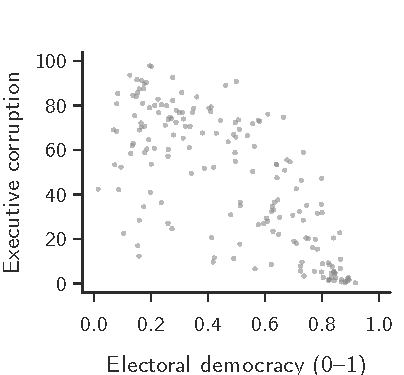
\includegraphics[width=0.95\linewidth]{poly_corr_1.pdf}
\end{figure}
\onslide<2|handout:0>
\begin{figure}[ht] \centering
        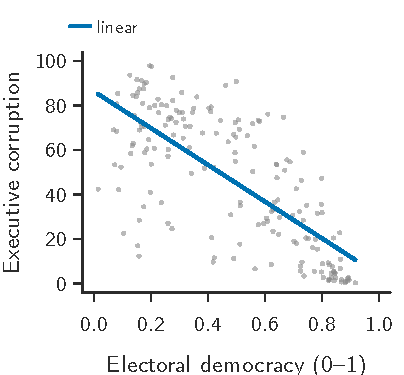
\includegraphics[width=0.95\linewidth]{poly_corr_2.pdf}
\end{figure}
\onslide<3|handout:1>
\begin{figure}[ht] \centering
        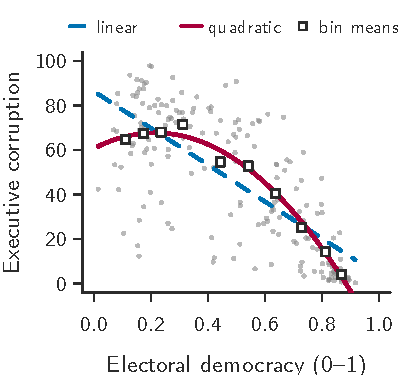
\includegraphics[width=0.95\linewidth]{poly_corr_3.pdf}
\end{figure}
\end{overprint}
\end{column}
\end{columns}
\slidesource{V-Dem v16, 2024 (executive corruption index $\times$ 100; electoral democracy index). Squares: mean corruption in each tenth of the countries, sorted by democracy.}
}

\frame{
\frametitle{Polynomial Example: Corruption and Democracy}

\begin{columns} [T]
\begin{column}[]{9cm}
\begin{itemize}
\uncover<1->{\item $\widehat{Y} = 60.8 + 65.1 X_1 - 151.5 X_1^2$}
\uncover<2->{\item Is $\beta_1$ the marginal effect of democracy on corruption?}
\uncover<3->{\item No! The slope depends on the level of democracy:\\
$\frac{\partial \widehat{Y}}{\partial X_1} = \widehat{\beta}_1+2\,\widehat{\beta}_2\,X_1 $\\
Here it is positive at low democracy and turns more and more negative as democracy rises.
}
\uncover<4->{\item If $\beta_2 > 0$ we get a U-shape, and if $\beta_2 < 0$ we get an inverted U-shape.}
\uncover<5->{\item Maximum/Minimum occurs at $\frac{- \beta_1}{2\beta_2}$. Here the turning point is at $X_1\approx 0.215$. But the bin means show no real rise. They stay between 65 and 72 up to about 0.37, then fall to 4. So the data are roughly flat, then falling.}
\end{itemize}
\end{column}
\begin{column}[]{6cm}
\begin{overprint}
\onslide<1->
\begin{figure}[ht] \centering
        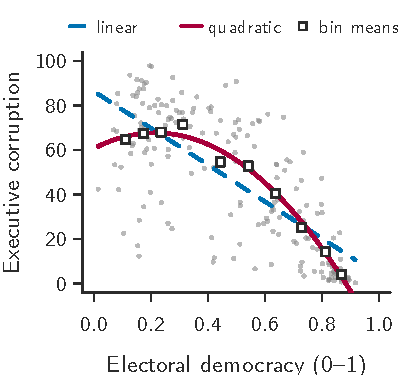
\includegraphics[width=0.95\linewidth]{poly_corr_3.pdf}
\end{figure}
\end{overprint}
\end{column}
\end{columns}
}

\frame{
\frametitle{Higher Order Polynomials}
\small
\begin{figure}[ht] \centering
        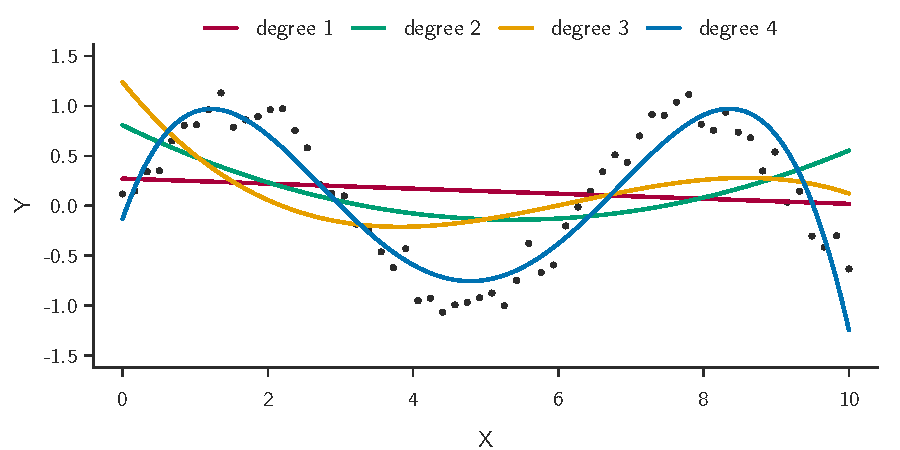
\includegraphics[height=0.70\textheight]{poly_sine_fits.pdf}
\end{figure}
Approximating data generated with a sine function. Red line is a first degree polynomial, green line is second degree, orange line is third degree and blue is fourth degree
}


\begin{frame}[fragile]
\frametitle{Dealing with Polynomials in R}
\begin{itemize}
  \item In R, you must enclose powers in a ``{\tt I()}'' construct inside a formula (here {\tt d} holds the 179 countries: {\tt execorr100} is executive corruption, {\tt polyarchy} electoral democracy):
\end{itemize}
\medskip
\spacingset{0.8}
\begin{Verbatim}[fontsize=\footnotesize, frame=single, label=R Code, commandchars=\\\{\}]
> summary(lm(execorr100 ~ polyarchy + \alert{I(}polyarchy^2\alert{)}, data = d))

Call:
lm(formula = execorr100 ~ polyarchy + I(polyarchy^2), data = d)

Residuals:
    Min      1Q  Median      3Q     Max
-54.973  -9.414   2.149  13.340  37.712

Coefficients:
               Estimate Std. Error t value Pr(>|t|)
(Intercept)      60.765      5.425  11.200  < 2e-16 ***
polyarchy        65.118     26.670   2.442   0.0156 *
I(polyarchy^2) -151.461     26.780  -5.656 6.17e-08 ***
---
Signif. codes:  0 *** 0.001 ** 0.01 * 0.05 . 0.1   1

Residual standard error: 18.92 on 176 degrees of freedom
Multiple R-squared:  0.6014,	Adjusted R-squared:  0.5969
F-statistic: 132.8 on 2 and 176 DF,  p-value: < 2.2e-16
\end{Verbatim}
\end{frame}

\end{document}
